%%%%%%%%%%%%%%%%%%%%%%%%%%%%%%%%%%%%%%%%%
% Classicthesis Typographic Thesis
% LaTeX Template
% Version 1.4 (1/1/16)
%
% This template has been downloaded from:
% http://www.LaTeXTemplates.com
%
% Original author:
% André Miede (http://www.miede.de) with commenting modifications by:
% Vel (vel@LaTeXTemplates.com)
%
% License:
% GNU General Public License (v2)
%
% General Tips:
% 1) Make sure to edit the classicthesis-config.file
% 2) New enumeration (A., B., C., etc in small caps): \begin{aenumerate} \end{aenumerate}
% 3) For margin notes: \marginpar or \graffito{}
% 4) Do not use bold fonts in this style, it is designed around them
% 5) Use tables as in the examples
% 6) See classicthesis-preamble.sty for useful commands
%
%%%%%%%%%%%%%%%%%%%%%%%%%%%%%%%%%%%%%%%%%

%----------------------------------------------------------------------------------------
%	PACKAGES AND OTHER DOCUMENT CONFIGURATIONS
%----------------------------------------------------------------------------------------

\documentclass[
		twoside,openright,titlepage,numbers=noenddot,headinclude,%1headlines,
	 	footinclude=true,cleardoublepage=empty,
		dottedtoc, % Make page numbers in the table of contents flushed right with dots leading to them
		BCOR=5mm,paper=a4,fontsize=11pt, % Binding correction, paper type and font size
		ngerman,american, % Languages, change this to your language(s)
		]{scrreprt} 
                
% Includes the file which contains all the document configurations and packages - make sure to edit this file
%%%%%%%%%%%%%%%%%%%%%%%%%%%%%%%%%%%%%%%%%
% Classicthesis Typographic Thesis
% Configuration File
%
% This file has been downloaded from:
% http://www.LaTeXTemplates.com
%
% Original author:
% André Miede (http://www.miede.de) with extensive commenting changes by:
% Vel (vel@LaTeXTemplates.com)
%
% License:
% GNU General Public License (v2)
%
% Important note:
% The main lines to change in this file are in the DOCUMENT VARIABLES
% section, the rest of the file is for advanced configuration.
%
%%%%%%%%%%%%%%%%%%%%%%%%%%%%%%%%%%%%%%%%%

%RSD: ADD PACKAGES AND DO YOUR OWN CONFIG TWEAKING HERE:
\usepackage{bm} % Might not be supported
\usepackage{amsmath}
\usepackage{ amssymb }

%%%%%%%%%%%%%%%%%%%%%%%%%%%%%%%%%%%%%%%%%%%%%%%%%%%%%%%%%


%\usepackage[euler-digits,euler-hat-accent]{eulervm}
\DeclareMathOperator{\argmax}{argmax}

%----------------------------------------------------------------------------------------
%	CHARACTER ENCODING
%----------------------------------------------------------------------------------------

\PassOptionsToPackage{utf8}{inputenc} % Set the encoding of your files. UTF-8 is the only sensible encoding nowadays. If you can't read äöüßáéçèê∂åëæƒÏ€ then change the encoding setting in your editor, not the line below. If your editor does not support utf8 use another editor!
\usepackage{inputenc}

%----------------------------------------------------------------------------------------
%	DOCUMENT VARIABLES
%	Fill in the lines below to enter your information into the thesis template
%	Each of the commands can be cited anywhere in the thesis
%----------------------------------------------------------------------------------------

% Remove drafting to get rid of the '[ Date - classicthesis version 4.0 ]' text at the bottom of every page
\PassOptionsToPackage{eulerchapternumbers,listings,drafting, pdfspacing, subfig,beramono,eulermath,parts}{classicthesis}
% Available options: drafting parts nochapters linedheaders eulerchapternumbers beramono eulermath pdfspacing minionprospacing tocaligned dottedtoc manychapters listings floatperchapter subfig

\newcommand{\myTitle}{Project Thesis in Nanotechnology at NTNU\xspace}
\newcommand{\mySubtitle}{Optimisation of Small Angle X-ray Scattering Tensor Tomography Gradient Descent Algorithm by Automatic Differentiation\xspace}
\newcommand{\myDegree}{Mr\xspace}
\newcommand{\myName}{Ruben Skjelstad Dragland\xspace}
\newcommand{\myProf}{Dag Werner Breiby\xspace}
\newcommand{\myOtherProf}{Basab Chattopadhyay\xspace}
\newcommand{\mySupervisor}{Dag Werner Breiby\xspace}
\newcommand{\myFaculty}{Faculty of Natural Sciences\xspace}
\newcommand{\myDepartment}{Department of Physics\xspace}
\newcommand{\myUni}{Norwegian University of Science and Technology\xspace}
\newcommand{\myLocation}{Trondheim\xspace}
\newcommand{\myTime}{December 2022\xspace}
\newcommand{\myVersion}{version 1.0\xspace}

%----------------------------------------------------------------------------------------
%	USEFUL COMMANDS
%----------------------------------------------------------------------------------------

\newcommand{\ie}{i.\,e.}
\newcommand{\Ie}{I.\,e.}
\newcommand{\eg}{e.\,g.}
\newcommand{\Eg}{E.\,g.}

\newcounter{dummy} % Necessary for correct hyperlinks (to index, bib, etc.)
\providecommand{\mLyX}{L\kern-.1667em\lower.25em\hbox{Y}\kern-.125emX\@}
\newlength{\abcd} % for ab..z string length calculation

%----------------------------------------------------------------------------------------
%	PACKAGES
%----------------------------------------------------------------------------------------

\usepackage{lipsum} % Used for inserting dummy 'Lorem ipsum' text into the template

%------------------------------------------------

%\PassOptionsToPackage{ngerman,american}{babel}  % Change this to your language(s)
% Spanish languages need extra options in order to work with this template
%\PassOptionsToPackage{spanish,es-lcroman}{babel}
\usepackage{babel}

%------------------------------------------------			

\usepackage{csquotes}
\PassOptionsToPackage{%
	%backend=biber, % Instead of bibtex
	backend=bibtex8,bibencoding=ascii,%
	language=auto,%
	style=numeric-comp,%
	%style=authoryear-comp, % Author 1999, 2010
	%bibstyle=authoryear,dashed=false, % dashed: substitute rep. author with ---
	sorting=nyt, % name, year, title
	maxbibnames=10, % default: 3, et al.
	%backref=true,%
	natbib=true % natbib compatibility mode (\citep and \citet still work)
}{biblatex}
\usepackage{biblatex}

%------------------------------------------------

\PassOptionsToPackage{fleqn}{amsmath} % Math environments and more by the AMS 
\usepackage{amsmath}

%------------------------------------------------

\PassOptionsToPackage{T1}{fontenc} % T2A for cyrillics
\usepackage{fontenc}

%------------------------------------------------

\usepackage{textcomp} % Fix warning with missing font shapes

%------------------------------------------------

\usepackage{scrhack} % Fix warnings when using KOMA with listings package  

%------------------------------------------------

\usepackage{xspace} % To get the spacing after macros right

%------------------------------------------------

\usepackage{mparhack} % To get marginpar right

%------------------------------------------------

\usepackage{fixltx2e} % Fixes some LaTeX stuff 

%------------------------------------------------

\PassOptionsToPackage{smaller}{acronym} % Include printonlyused in the first bracket to only show acronyms used in the text
\usepackage{acronym} % Nice macros for handling all acronyms in the thesis

%\renewcommand*{\acsfont}[1]{\textssc{#1}} % For MinionPro
\renewcommand*{\aclabelfont}[1]{\acsfont{#1}}

%------------------------------------------------

\PassOptionsToPackage{pdftex}{graphicx}
\usepackage{graphicx}

%----------------------------------------------------------------------------------------
%	FLOATS: TABLES, FIGURES AND CAPTIONS SETUP
%----------------------------------------------------------------------------------------

\usepackage{tabularx} % Better tables
\setlength{\extrarowheight}{3pt} % Increase table row height
\newcommand{\tableheadline}[1]{\multicolumn{1}{c}{\spacedlowsmallcaps{#1}}}
\newcommand{\myfloatalign}{\centering} % To be used with each float for alignment
\usepackage{caption}
\captionsetup{font=small}
\usepackage{subfig}

%----------------------------------------------------------------------------------------
%	CODE LISTINGS SETUP
%----------------------------------------------------------------------------------------

\usepackage{listings}
%\lstset{emph={trueIndex,root},emphstyle=\color{BlueViolet}}%\underbar} % For special keywords
\lstset{language=[LaTeX]Tex,%C++ % Specify the language(s) for listings here
	morekeywords={PassOptionsToPackage,selectlanguage},
	keywordstyle=\color{RoyalBlue}, % Add \bfseries for bold
	basicstyle=\small\ttfamily, % Makes listings a smaller font size and a different font
	%identifierstyle=\color{NavyBlue}, % Color of text inside brackets
	commentstyle=\color{Green}\ttfamily, % Color of comments
	stringstyle=\rmfamily, % Font type to use for strings
	numbers=left, % Change left to none to remove line numbers
	numberstyle=\scriptsize, % Font size of the line numbers
	stepnumber=5, % Increment of line numbers
	numbersep=8pt, % Distance of line numbers from code listing
	showstringspaces=false, % Sets whether spaces in strings should appear underlined
	breaklines=true, % Force the code to stay in the confines of the listing box
	%frameround=ftff, % Uncomment for rounded frame
	%frame=single, % Frame border - none/leftline/topline/bottomline/lines/single/shadowbox/L
	belowcaptionskip=.75\baselineskip % Space after the "Listing #: Desciption" text and the listing box
}

%----------------------------------------------------------------------------------------
%	HYPERREFERENCES
%----------------------------------------------------------------------------------------

\PassOptionsToPackage{pdftex,hyperfootnotes=false,pdfpagelabels}{hyperref}
\usepackage{hyperref}  % backref linktocpage pagebackref
\pdfcompresslevel=9
\pdfadjustspacing=1

\hypersetup{
	% Uncomment the line below to remove all links (to references, figures, tables, etc), useful for b/w printouts
	%draft, 
	colorlinks=true, linktocpage=true, pdfstartpage=3, pdfstartview=FitV,
	% Uncomment the line below if you want to have black links (e.g. for printing black and white)
	%colorlinks=false, linktocpage=false, pdfborder={0 0 0}, pdfstartpage=3, pdfstartview=FitV, 
	breaklinks=true, pdfpagemode=UseNone, pageanchor=true, pdfpagemode=UseOutlines,%
	plainpages=false, bookmarksnumbered, bookmarksopen=true, bookmarksopenlevel=1,%
	hypertexnames=true, pdfhighlight=/O,%nesting=true,%frenchlinks,%
	urlcolor=webbrown, linkcolor=RoyalBlue, citecolor=webgreen, %pagecolor=RoyalBlue,%
	%urlcolor=Black, linkcolor=Black, citecolor=Black, %pagecolor=Black,%
	%------------------------------------------------
	% PDF file meta-information
	pdftitle={\myTitle},
	pdfauthor={\textcopyright\ \myName, \myUni, \myFaculty},
	pdfsubject={},
	pdfkeywords={},
	pdfcreator={pdfLaTeX},
	pdfproducer={LaTeX with hyperref and classicthesis}
	%------------------------------------------------
}

%----------------------------------------------------------------------------------------
%	AUTOREFERENCES SETUP
%	Redefines how references in text are prefaced for different 
%	languages (e.g. "Section 1.2" or "section 1.2")
%----------------------------------------------------------------------------------------

\makeatletter
\@ifpackageloaded{babel}
{
	\addto\extrasamerican{
		\renewcommand*{\figureautorefname}{Figure}
		\renewcommand*{\tableautorefname}{Table}
		\renewcommand*{\partautorefname}{Part}
		\renewcommand*{\chapterautorefname}{Chapter}
		\renewcommand*{\sectionautorefname}{Section}
		\renewcommand*{\subsectionautorefname}{Section}
		\renewcommand*{\subsubsectionautorefname}{Section}
	}
	\addto\extrasngerman{
		\renewcommand*{\paragraphautorefname}{Absatz}
		\renewcommand*{\subparagraphautorefname}{Unterabsatz}
		\renewcommand*{\footnoteautorefname}{Fu\"snote}
		\renewcommand*{\FancyVerbLineautorefname}{Zeile}
		\renewcommand*{\theoremautorefname}{Theorem}
		\renewcommand*{\appendixautorefname}{Anhang}
		\renewcommand*{\equationautorefname}{Gleichung}
		\renewcommand*{\itemautorefname}{Punkt}
	}
	\providecommand{\subfigureautorefname}{\figureautorefname} % Fix to getting autorefs for subfigures right
}{\relax}
\makeatother

%----------------------------------------------------------------------------------------

\usepackage{classicthesis}

%----------------------------------------------------------------------------------------
%	CHANGING TEXT AREA 
%----------------------------------------------------------------------------------------

%\linespread{1.05} % a bit more for Palatino
%\areaset[current]{312pt}{761pt} % 686 (factor 2.2) + 33 head + 42 head \the\footskip
%\setlength{\marginparwidth}{7em}%
%\setlength{\marginparsep}{2em}%

%----------------------------------------------------------------------------------------
%	USING DIFFERENT FONTS
%----------------------------------------------------------------------------------------

%\usepackage[oldstylenums]{kpfonts} % oldstyle notextcomp
%\usepackage[osf]{libertine}
%\usepackage[light,condensed,math]{iwona}
%\renewcommand{\sfdefault}{iwona}
%\usepackage{lmodern} % <-- no osf support :-(
%\usepackage{cfr-lm} % 
%\usepackage[urw-garamond]{mathdesign} <-- no osf support :-(
%\usepackage[default,osfigures]{opensans} % scale=0.95 
%\usepackage[sfdefault]{FiraSans}

\addbibresource{Bibliography.bib} % The file housing your bibliography
%\addbibresource[label=ownpubs]{Self_Publications.bib} % Uncomment for optional self-publications

%\hyphenation{Put special hyphenation here}

\begin{document}

\frenchspacing % Reduces space after periods to make text more compact

\raggedbottom % Makes all pages the height of the text on that page

\selectlanguage{american} % Select your default language - e.g. american or ngerman

%\renewcommand*{\bibname}{new name} % Uncomment to change the name of the bibliography
%\setbibpreamble{} % Uncomment to include a preamble to the bibliography - some text before the reference list starts

\pagenumbering{roman} % Roman page numbering prior to the start of the thesis content (i, ii, iii, etc)

\pagestyle{plain} % Suppress headers for the pre-content pages

%----------------------------------------------------------------------------------------
%	PRE-CONTENT THESIS PAGES
%----------------------------------------------------------------------------------------

% Title Page

\begin{titlepage}

    \begin{addmargin}[-1cm]{-3cm}
        \begin{center}
            \large

            \hfill
            \vfill

            \begingroup
            \color{Maroon}\spacedallcaps{\myTitle} \\ \bigskip % Thesis title
            \endgroup

            \spacedlowsmallcaps{\myName} % Your name

            \vfill

            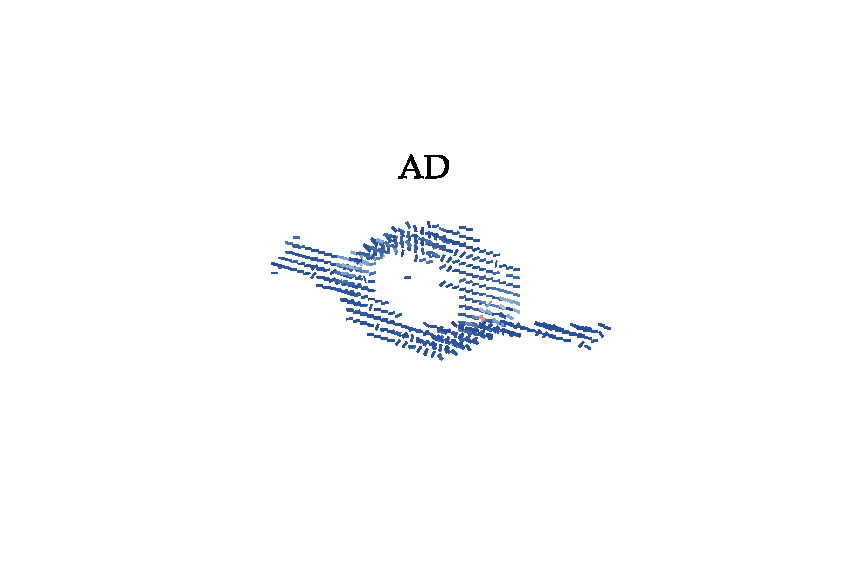
\includegraphics[trim={3.5cm 3.5cm 3.5cm 3.5cm},clip, width=10cm]{./svg-inkscape/ck_indAD_svg-tex.pdf} \\ \medskip % Picture

            \mySubtitle \\ \medskip % Thesis subtitle
            %\myDegree \\
            %\myDepartment \\
            %\myFaculty \\
            %\myUni \\ \bigskip

            \myTime\ -- \myVersion % Time and version

            \vfill

        \end{center}
    \end{addmargin}

\end{titlepage} % Main title page

% Back of the title page

\thispagestyle{empty}

\hfill

\vfill

\noindent\myName: \textit{\myTitle,} \mySubtitle, %\myDegree, 
\textcopyright\ \myTime

% You may wish to do something with the back of the title page, such as including your supervisors, location or time frame of the work. Below is an example of doing so although you may want to tweak it to your liking.

\bigskip

\noindent\spacedlowsmallcaps{Supervisors}: \\
\myProf \\
\myOtherProf \\ 
%\mySupervisor

%\medskip \\

%\noindent\spacedlowsmallcaps{Location}: \\
%\myLocation

%\medskip \\

%\noindent\spacedlowsmallcaps{Time Frame}: \\
%\myTime
 % Back of the title page

\cleardoublepage% Dedication

\thispagestyle{empty}
\refstepcounter{dummy}

\pdfbookmark[1]{Dedication}{Dedication} % Bookmark name visible in a PDF viewer

\vspace*{3cm}

\begin{center}
\emph{Ohana} means family. \\
Family means nobody gets left behind, or forgotten. \\ \medskip
--- Lilo \& Stitch    
\end{center}

\medskip

\begin{center}
Dedicated to the loving memory of Rudolf Miede. \\ \smallskip
1939\,--\,2005
\end{center}

% What is dedication? % Dedication page

%\cleardoublepage\include{FrontBackMatter/Foreword} % Uncomment and create a Foreword.tex to include a foreword

\cleardoublepage% Abstract

%\renewcommand{\abstractname}{Abstract} % Uncomment to change the name of the abstract

\pdfbookmark[1]{Abstract}{Abstract} % Bookmark name visible in a PDF viewer

\begingroup
\let\clearpage\relax
\let\cleardoublepage\relax
\let\cleardoublepage\relax

\chapter*{Abstract}
Short summary of the contents\dots a great guide by 
Kent Beck how to write good abstracts can be found here:  
\begin{center}
\url{https://plg.uwaterloo.ca/~migod/research/beckOOPSLA.html}
\end{center}

\endgroup			

\vfill % Abstract page

\cleardoublepage% Publications - a page listing research articles written using content in the thesis

\pdfbookmark[1]{Publications}{Publications} % Bookmark name visible in a PDF viewer

\chapter*{Publications} % Publications page text

Some ideas and figures have appeared previously in the following publications:\\

\noindent Put your publications from the thesis here. The packages \texttt{multibib} or \texttt{bibtopic} etc. can be used to handle multiple different bibliographies in your document.

%\begin{refsection}[ownpubs]
%    \small
%    \nocite{*} % is local to to the enclosing refsection
%    \printbibliography[heading=none]
%\end{refsection}

%\emph{Attention}: This requires a separate run of \texttt{bibtex} for your \texttt{refsection}, \eg, \texttt{ClassicThesis1-blx} for this file. You might also use \texttt{biber} as the backend for \texttt{biblatex}. See also \url{http://tex.stackexchange.com/questions/128196/problem-with-refsection}. % Publications from the thesis page

\cleardoublepage% Acknowledgements

\pdfbookmark[1]{Acknowledgements}{Acknowledgements} % Bookmark name visible in a PDF viewer

% \begin{flushright}{\slshape    
% We have seen that computer programming is an art, \\ 
% because it applies accumulated knowledge to the world, \\ 
% because it requires skill and ingenuity, and especially \\
% because it produces objects of beauty.} \\ \medskip
% --- \defcitealias{knuth:1974}{Donald E. Knuth}\citetalias{knuth:1974} \citep{knuth:1974}
% \end{flushright}

\bigskip

%----------------------------------------------------------------------------------------

\begingroup

\let\clearpage\relax
\let\cleardoublepage\relax
\let\cleardoublepage\relax

\chapter*{Acknowledgements}

% \noindent Put your acknowledgements here.\\
% 
% \noindent Many thanks to everybody who already sent me a postcard!\\
% 
% \noindent Regarding the typography and other help, many thanks go to Marco Kuhlmann, Philipp Lehman, Lothar Schlesier, Jim Young, Lorenzo Pantieri and Enrico Gregorio\footnote{Members of GuIT (Gruppo Italiano Utilizzatori di \TeX\ e \LaTeX )}, J\"org Sommer, Joachim K\"ostler, Daniel Gottschlag, Denis Aydin, Paride Legovini, Steffen Prochnow, Nicolas Repp, Hinrich Harms, Roland Winkler, and the whole \LaTeX-community for support, ideas and some great software.
% 
% \bigskip
% 
% \noindent\emph{Regarding \mLyX}: The \mLyX\ port was initially done by
% \emph{Nicholas Mariette} in March 2009 and continued by
% \emph{Ivo Pletikosi\'c} in 2011. Thank you very much for your work and the contributions to the original style.

\endgroup % Acknowledgements page

\pagestyle{scrheadings} % Show chapter titles as headings

\cleardoublepage% Table of Contents - List of Tables/Figures/Listings and Acronyms

\refstepcounter{dummy}

\pdfbookmark[1]{\contentsname}{tableofcontents} % Bookmark name visible in a PDF viewer

\setcounter{tocdepth}{2} % Depth of sections to include in the table of contents - currently up to subsections

\setcounter{secnumdepth}{3} % Depth of sections to number in the text itself - currently up to subsubsections

\manualmark
\markboth{\spacedlowsmallcaps{\contentsname}}{\spacedlowsmallcaps{\contentsname}}
\tableofcontents 
\automark[section]{chapter}
\renewcommand{\chaptermark}[1]{\markboth{\spacedlowsmallcaps{#1}}{\spacedlowsmallcaps{#1}}}
\renewcommand{\sectionmark}[1]{\markright{\thesection\enspace\spacedlowsmallcaps{#1}}}

\clearpage

\begingroup 
\let\clearpage\relax
\let\cleardoublepage\relax
\let\cleardoublepage\relax

%----------------------------------------------------------------------------------------
%	List of Figures
%----------------------------------------------------------------------------------------

\refstepcounter{dummy}
%\addcontentsline{toc}{chapter}{\listfigurename} % Uncomment if you would like the list of figures to appear in the table of contents
\pdfbookmark[1]{\listfigurename}{lof} % Bookmark name visible in a PDF viewer

\listoffigures

\vspace{8ex}
\newpage

%----------------------------------------------------------------------------------------
%	List of Tables
%----------------------------------------------------------------------------------------

\refstepcounter{dummy}
%\addcontentsline{toc}{chapter}{\listtablename} % Uncomment if you would like the list of tables to appear in the table of contents
\pdfbookmark[1]{\listtablename}{lot} % Bookmark name visible in a PDF viewer

\listoftables
        
\vspace{8ex}
\newpage
    
%----------------------------------------------------------------------------------------
%	List of Listings
%---------------------------------------------------------------------------------------- 

\refstepcounter{dummy}
%\addcontentsline{toc}{chapter}{\lstlistlistingname} % Uncomment if you would like the list of listings to appear in the table of contents
\pdfbookmark[1]{\lstlistlistingname}{lol} % Bookmark name visible in a PDF viewer

\lstlistoflistings 

\vspace{8ex}
\newpage
       
%----------------------------------------------------------------------------------------
%	Acronyms
%----------------------------------------------------------------------------------------

\refstepcounter{dummy}
%\addcontentsline{toc}{chapter}{Acronyms} % Uncomment if you would like the acronyms to appear in the table of contents
\pdfbookmark[1]{Acronyms}{acronyms} % Bookmark name visible in a PDF viewer

\markboth{\spacedlowsmallcaps{Acronyms}}{\spacedlowsmallcaps{Acronyms}}

\chapter*{Acronyms}

\begin{acronym}[UML]
\acro{DRY}{Don't Repeat Yourself}
\acro{API}{Application Programming Interface}
\acro{UML}{Unified Modeling Language}
\acro{FBP}{Filtered Back Projection}
\acro{CT}{Computed Tomography}
\acro{ML}{Maximum-Likelihood}
\acro{GD}{Gradient Descent}
\acro{CGD}{Conjugated Gradient Descent}
\acro{AD}{Automatic Differentiation}
\acro{SAXSTT}{Small Angle X-ray Scattering Tensor Tomography}
\acro{SH}{Spherical Harmonics}

\end{acronym}  
                   
\endgroup % Contents, list of figures/tables/listings and acronyms

\cleardoublepage

\pagenumbering{arabic} % Arabic page numbering for thesis content (1, 2, 3, etc)
%\setcounter{page}{90} % Uncomment to manually start the page counter at an arbitrary value (for example if you wish to count the pre-content pages in the page count)

\cleardoublepage % Avoids problems with pdfbookmark


%%% RSD: Copied from the file that does not compile. Hope this manages this now. 
%----------------------------------------------------------------------------------------
%	THESIS CONTENT - CHAPTERS
%----------------------------------------------------------------------------------------

%\ctparttext{You can put some informational part preamble text here. Illo principalmente su nos. Non message \emph{occidental} angloromanic da. Debitas effortio simplificate sia se, auxiliar summarios da que, se avantiate publicationes via. Pan in terra summarios, capital interlingua se que. Al via multo esser specimen, campo responder que da. Le usate medical addresses pro, europa origine sanctificate nos se.} % Text on the Part 1 page describing  the content in Part 1

%\ctparttext{\chapter{Introduction}

Machine learning has grown to be a powerful tool in many disciplines within physics. This includes computed tomography...}
%\ctparttext{Machine learning has grown to be a powerful tool in many disciplines within physics. This includes computed tomography...} Not include

\part{Introduction} %\part{Some Kind of Manual} % First part of the thesis

\chapter{Introduction}


Machine learning has grown to be a powerful tool, and is applied to many aspects of society,
either through marketing of commercial products, or in the development of new technologies aimed at easing the lives of people.
However, there is also an ongoing revolution in the field of physics,
where machine learning is used to solve complex optimisation tasks, thereby revealing new insights that were previously nonextractable.
One instance where machine learning has been proven to be powerful is within the field of computed tomography (CT) and related algorithms thereof.
CT is known as a medical imaging technique that uses X-rays to produce a 3D image of the internal objects of the patient that was scanned.
The technique is also highly applicable to materials science, where micro-CT ($\mu CT$) is being used to image the internal structure of microporous materials.
However, the term computed tomography refers actually to a broader class of algorithms where 3D models are reconstructed from projections.
One of these algorithms is called Small Angle X-ray Scattering Tensor Tomography (SAXSTT), which distinguishes itself from conventional CT by the fact that the technique
reconstructs a 3D vector field based on X-ray scattering measurements. Conventional CT reconstructs, as mentioned, a 3D scalar field from X-ray absorption measurements.
SAXSTT is therefore able to do harmless and efficient orientation mapping of uniaxial nanostructures throughout any three-dimensional amorphous sample with micrometer spatial resolution.
The technique combines the power of gradient descent with the quantum mechanical relations between scattering pattern and real-space orientation.

In this thesis, optimisation of Small Angle Scattering X-ray Tensor Tomography is investigated.
The algorithm is still young and has not yet been developed to its full potential.
One important tool in the continued development of this algorithm is automatic differentiation.
Therefore, the first step in this project work is to implement the gradient calculation of the SAXSTT algorithm using automatic differentiation.
With this in place, the reconstruction technique can be optimised and expanded in a versatile and efficient manner.
An initial demonstration of such optimisation is also presented in this thesis, by testing an alternative functional to model the 3D reciprocal space map. % Chapter 1

\cleardoublepage % Empty page before the start of the next part

%------------------------------------------------

\ctparttext{You can put some informational part preamble text here. Illo principalmente su nos. Non message \emph{occidental} angloromanic da. Debitas effortio simplificate sia se, auxiliar summarios da que, se avantiate publicationes via. Pan in terra summarios, capital interlingua se que. Al via multo esser specimen, campo responder que da. Le usate medical addresses pro, europa origine sanctificate nos se.} % Text on the Part 2 page describing the content in Part 2

\part{Review of The Literature}%\part{The Showcase} % Second part of the thesis

%
\chapter{Computed Tomography}

%RSD: Should do more precise calculations?
\section{X-rays}
X-rays are electromagnetic waves with energy in the orders of $keV$. From Planck's Equation \eqref{eq:Plancks_eq}, this corresponds to nanometer wavelengths. The equation relates energy of a photon $E$ to the frequency $\nu$ or wavelength $\lambda$ of the corresponding electromagnetic wave, as

\begin{equation}\label{eq:Plancks_eq}
    E = 2\pi \hbar \nu, \newline
    
    \nu = \frac{c}{\lambda},
\end{equation}
\noindent
with $c \sim 2.99776 \times 10^8 m/s$ being the speed of light \cite{blokhin1961physics}. The other constant is the reduced Planck's constant $\hbar \sim 1.0543 \times 10^{-34} Js$. 

Excitation, acceleration, and deceleration are the three most commonly utilised processes for producing X-rays. The first method is commonly referred to as "Characteristic X-ray radiation", which occurs when a highly energetic electron collides into a target atom. The accelerated electron transfers enough energy to eject an inner-shell electron from the atom. An outer electron may therefore occupy a lower-energy state. Due to conservation of energy, this process causes emission of a photon, as illustrated in Equation \eqref{eq:Char_radiation}. As the atomic energy levels are discrete, this process is characterised by a spectrum of discrete X-ray emission lines.
%\cite{Stark, G.. "X-ray." Encyclopedia Britannica, January 30, 2020. https://www.britannica.com/science/X-ray.}.  

\begin{equation}\label{eq:Char_radiation}
    E_{\mathrm{photon}} = - \Delta E = - (E_f - E_i)
\end{equation}

In addition to excitation, scattering events occur when electrons pass through an anode material. These events accelerate the electrons in a new direction, and X-rays known as $"Bremsstrahluhng"$ are emitted. % Include Intensity relation of Bremsstrahlung?

%Improve, Figure or equations
The synchrotron is the last common form of X-ray production, and is also based upon the principle of $"Bremsstrahluhng"$. Generally, charged particles are accelerated to very high energies, and magnets maintain their circular path. As moving objects in a circular path experience a centrifugal acceleration perpendicular to its directions, $"Bremsstrahluhng"$ X-rays are emitted. 
%\cite{Britannica, T. Editors of Encyclopaedia. "synchrotron." Encyclopedia Britannica, February 7, 2018. https://www.britannica.com/technology/synchrotron.}

\section{Beer-Lambert's Law}
The intensity of X-rays attenuates upon interacting with matter. This is due to photoelectric absorption, elastic Rayleigh scattering, and inelastic Compton scattering. The attenuation coefficient $\mu$ describes this attenuation in an inhomogeneous sample as
% Include formulas for scattering processes?

\begin{equation}
    I(s) = I(0) \exp(- \int_{0}^{s} \mu(\nu) d\nu),
\end{equation}
\noindent
where $s$ is the distance from the initial intensity to the end of the sample, effectively the thickness of the sample, and $I(0)$ is the initial intensity. Here, the spectral dependence, $\mu(E,\nu)$ is often neglected as it is unknown \cite{buzug2009computed}. A simple manipulation of the expression gives the projection line integral

\begin{equation}\label{eq:projection}
    p(s) = -\ln(\frac{I(s)}{I(0)} ) = \int_{0}^{s} \mu(\nu) d\nu.
\end{equation}

\section{Radon Transform}
The projection line integral in Equation \eqref{eq:projection} may be viewed as a Radon transform of an object function $f(x,y)$ for a single orientation $\theta$ \cite{zeng2010medical}. Confidence in this statement may be achieved by comparing Equation \eqref{eq:projection} with a single-angle Radon transform \eqref{eq:Radon_transform}

\begin{equation}\label{eq:Radon_transform}
    p_{\theta}(r) = \int_{-\infty}^{\infty} f(r,\nu) d\nu.
\end{equation}

%\section{Detectors}??? Cannot be relevant

\section{Fourier Slice Theorem}
%\section{Projections}
The key in computed tomography is to determine the spatial dependence of the attenuation coefficient. By sampling many projections, meaning line integrals from different orientations and crossections, data necessary to reconstruct a three-dimensional image is collected. For a given crossection of the object $f(x,y)$, the detected intensity is plotted as a function of projection number and pixel number in what is called a sinogram. By utilising this sinogram and the Fourier slice theorem, the object $f(x,y)$ may be determined by other means than computing the full inverse Radon transform.

%\section{Fourier Slice Theorem}

The Fourier slice theorem states that the full 2D Fourier transform $F(\omega_x, \omega_y)$ of an object $f(x,y)$ can be constructed from a series of 1D Fourier transforms $P(\omega)$ of projections $p(s)$ with different orientations \cite{zeng2010medical}. 
%  that the 1D Fourier transform $P(\omega)$ of the projection $p(s)$ of the object $f(x,y)$ is equal to a slice through the origin of the 2D Fourier transform $F(\omega_x, \omega_y)$ \cite{}. 


% ILLUSTRATE with a Figure
%See and reconstruct Figure 5.13 in buzug2009computed possibly... or the one in zeng2010medical


\section{Filtered Back Projection}
In short, the filtered back projection (FBP) algorithm reconstructs the object by forward and inverse Fourier transforms. Firstly, the sinogram of projections is mapped to frequency space in polar coordinates by subsequent 1D Fourier transforms, as shown in Equation \eqref{eq:FBP_1}:

\begin{equation}\label{eq:FBP_1}
    P(\theta, \omega) = \int_{-\infty}^{\infty} p(\theta,r)e^{-2\pi i\omega r} dr.
\end{equation}

With this the 2D Fourier transform $F(u,v)$ of the object $f(x,y)$ is found. The final step is an inverse 2D Fourier transform with a $ramp$-filter of $|\omega|$ to account for the radial distribution of points in polar coordinates. This filter is also the Jacobian of the area integration element in the polar Fourier space. Consequently, the object function can be expressed as

\begin{equation}
    f(x,y) = \int_{0}^{\pi} \int_{-\infty}^{\infty} \left|\omega\right| P(\theta,\omega)e^{-2\pi i\omega (x\cos\theta - y\sin\theta)} d\omega d\theta.
\end{equation}

%RSD: Read through a couple of times. 







%\include{2.Teil Theory/02TheorySAXSTT} 
%\include{2.Teil Theory/03MachineLearning} 
%\include{2.Teil Theory/04GradientDescent}
%\include{2.Teil Theory/05TheoryAutodiff}
% This is many chapters. Instead, one chapter on the image technique and one on the optimalisation?

\chapter{Computed Tomography}

%RSD: Should do more precise calculations?
\section{X-rays}\label{sec:CT_Xrays}

X-rays are electromagnetic waves with energy in the orders of $keV$. Planck's Equation,
\begin{equation}\label{eq:Plancks_eq}
    E = \hslash \omega = 2\pi \hslash \frac{c}{\lambda},
\end{equation}
\noindent
relates the energy of a photon $E$ to the angular frequency $\omega$ or wavelength $\lambda$ of the corresponding electromagnetic wave.
$c = 2.99792 \times 10^8 m/s$ is the speed of light.
The other constant is the reduced Planck's constant $\hslash = 1.0543 \times 10^{-34} Js$  \cite{blokhin1961physics}.
Whence, X-rays typically have wavelengths in the sub-nanometer range.


Excitation and acceleration are the most common phenomena where X-ray radiation occurs.
X-ray radiation from excitation, called "Characteristic X-ray radiation", occurs when a highly energetic electron collides into a target atom.
The accelerated electron transfers enough energy to eject an inner-shell electron with energy $E_i$,
and an outer electron with energy $E_f$ lowers its energy-state by filling the vacancy,

\begin{equation}\label{eq:Char_radiation}
    E_{\mathrm{photon}} = - \Delta E = - (E_f - E_i).
\end{equation}

Due to conservation of energy, this process causes emission of a photon, as described in Equation \eqref{eq:Char_radiation}.
As the atomic energy levels are discrete, this process gives rise to a spectrum of discrete X-ray emission lines.
%\cite{Stark, G.. "X-ray." Encyclopedia Britannica, January 30, 2020. https://www.britannica.com/science/X-ray.}.


Additionally, scattering events occur when electrons pass through an anode material.
These events accelerate the electrons in new directions, and X-rays known as $"Bremsstrahluhng"$ are emitted. % Include Intensity relation of Bremsstrahlung?

%Improve, Figure or equations
The synchrotron is the last common X-ray source.
Generally, charged particles are accelerated to very high velocities, and magnets exert forces on the charged particles, which in turn cause acceleration, in accordance with
Lorentz force and Newton's second law of motion,

\begin{equation}\label{eq:Lorentz_force}
    m\vectorBU{a} = q \vectorBU{v} \times \vectorBU{B}.
\end{equation}
As described, the acceleration will be parallel to the cross product between the velocity $\vectorBU{v}$ and the external magnetic field $\vectorBU{B}$ \cite{}. %RSD: Cite
%\cite{Britannica, T. Editors of Encyclopaedia. "synchrotron." Encyclopedia Britannica, February 7, 2018. https://www.britannica.com/technology/synchrotron.}
% Add equation?


\section{Beer-Lambert's Law}
The X-ray beam intensity attenuates upon interacting with matter due to photoelectric absorption, elastic Rayleigh scattering, and inelastic Compton scattering.
The attenuation coefficient $\mu$ describes this attenuation in an inhomogeneous sample as

\begin{equation}
    I(s) = I(0) \exp(- \int_{0}^{s} \mu(\nu) d\nu),
\end{equation}
\noindent
where $s$ is the thickness of the sample, and $I(0)$ is the initial intensity. The spectral dependence $\mu(\nu)$ is here neglected, as it often is, as the beam is assumed to be almost fully monochromatic \cite{buzug2009computed}.
A simple manipulation of the expression gives the projection line integral

\begin{equation}\label{eq:projection}
    p(s) = -\ln(\frac{I(s)}{I(0)} ) = \int_{0}^{s} \mu(\nu) d\nu.
\end{equation}

%RSD: Rewrite. 
\section{Radon Transform}
The projection line integral in Equation \eqref{eq:projection} is closely related to the Radon transform of an object function $f(x,y)$ for a single orientation $\theta$ \cite{zeng2010medical}.
Confidence in this statement may be achieved by comparing Equation \eqref{eq:projection} with a single-angle Radon transform,

\begin{equation}\label{eq:Radon_transform}
    p_{\theta}(r) = \int_{-\infty}^{\infty} f(r,\nu) d\nu.
\end{equation}
Collected Radon transform data is called a sinogram, and is used to reconstruct the original object function $f(x,y)$ \cite{gonzalez2018digital}.
%The Radon transform of a function $f(x,y)$ along the angle $\theta$ is defined in Equation \eqref{eq:Radon_transform} purely as a line integral along the desired angle. %?

%\section{Detectors}??? Cannot be relevant

\section{Fourier Slice Theorem}
%\section{Projections}
The key in computed tomography is to determine the spatial dependency of the attenuation coefficient $\mu(\bm{r})$.
By sampling many projections, meaning line integrals from different orientations, data necessary to reconstruct a three-dimensional image is collected.
For a given cross-section of the sample $f(x, y)$, the detected intensity is plotted as a function of projection number and detector number in what is called a sinogram.
By utilising this sinogram and the Fourier slice theorem, the object $f(x, y)$ may be determined by other means than computing the full inverse Radon transform.
%\section{Fourier Slice Theorem}

The Fourier slice theorem states that the Fourier transform of a projection
is a slice of the 2D Fourier Transform of the region from which the projection was obtained \cite{gonzalez2018digital}.
Consequently, the full 2D Fourier transform
$F(\omega_x, \omega_y)$ of an object $f(x,y)$ can be constructed from a series of 1D Fourier transforms
$P(\omega)$ of projections $p(s)$ with different orientations \cite{zeng2010medical}.
In other words, the Fourier transform of a single projection makes up one angle of the full 2D Fourier transform,

\begin{equation}\label{eq:Fourier_slice}
    P(\theta, \omega) = F \left( \omega \cos \theta, -\omega \sin \theta \right). %\int_{-\infty}^{\infty} P(\omega) e^{i \omega_x x} dx.
\end{equation}
%  that the 1D Fourier transform $P(\omega)$ of the projection $p(s)$ of the object $f(x,y)$ is equal to a slice through the origin of the 2D Fourier transform $F(\omega_x, \omega_y)$ \cite{}. 


% ILLUSTRATE with a Figure
%See and reconstruct Figure 5.13 in buzug2009computed possibly... or the one in zeng2010medical


\section{Filtered Back Projection}
In short, the filtered back projection (FBP) algorithm reconstructs the object by forward and inverse Fourier transforms.
Firstly, the sinogram of projections is mapped to frequency space in polar coordinates by subsequent 1D Fourier transforms, mathematically described as:

\begin{equation}\label{eq:FBP_1}
    P(\theta, \omega) = \int_{-\infty}^{\infty} p(\theta,r)e^{-2\pi i\omega r} dr.
\end{equation}

With this the 2D Fourier transform $F(u,v)$ of the object $f(x,y)$ is found.
The final step is an inverse 2D Fourier transform with, for instance, a $ramp$-filter of $|\omega|$ to account for the radial distribution of points in polar coordinates.
This filter is also the Jacobian of the area integration element in the polar Fourier space.
Consequently, the object function can be expressed as

\begin{equation}
    f(x,y) = \int_{0}^{\pi} \int_{-\infty}^{\infty} \left|\omega\right| P(\theta,\omega)e^{-2\pi i\omega (x\cos\theta - y\sin\theta)} d\omega d\theta.
\end{equation}

%RSD: Read through a couple of times. 







\chapter{Machine Learning Optimisation}
\label{ch:optimisation}

\section{Maximum Likelihood Estimation}


The maximum likelihood estimator is defined to be the set of parameters $\vectorgreek{\theta}_{ML}$ that maximise the probability $P(\vectorBU{y} \mid \vectorBU{x}; \vectorgreek{\theta})$.
In other words, it chooses the parameters that produce the most probable estimation $\vectorBU{\widehat{y}}$ of the true output $\vectorBU{y}$ given the input $\vectorBU{x}$.
Mathematically, the maximum likelihood estimator is defined as

\begin{equation}\label{eq:Max_likelihood}
    \vectorgreek{\theta}_{ML} = \argmax_{\vectorgreek{\theta}} P(\vectorBU{y} \mid \vectorBU{x}; \vectorgreek{\theta}),
\end{equation}
\noindent
where $\argmax_{\vectorgreek{\theta}}$ returns the arguments that maximise the probability.

ML estimation is an example of supervised learning, because the true output, called the targets, are known.
In supervised learning, the estimation is evaluated by computing the error relative to the true output.
The expression for the total error of the model is called the cost function $J(\vectorgreek{\theta})$,
which is a sum of loss functions $\mathcal{L}(\vectorBU{y},\vectorBU{\widehat{y}} )$ representing the error of a single data point.

\section{Gradient Descent}

Gradient descent is an optimisation algorithm that updates the model's parameters based on the gradient of the cost function and the step size $\alpha$ \cite{ruder2016overview}.
After each backward pass, the parameters of the model are updated according to the following equation:

\begin{equation}\label{eq:GD}
    \vectorgreek{\theta} = \vectorgreek{\theta} - \alpha \bm{\nabla_{\theta}} J(\vectorgreek{\theta}).
\end{equation}

The idea of this algorithm is that by following the gradient of the cost function,
the estimation will converge to the correct solution of the problem,
which naturally results in the minimal error.
Gradient descent in parameter space is visualised in Figure \ref{fig:GD_surface}
% Matplotlib surface plot with path. + Make gif. 

\begin{figure}[h!]
    \centering
    %\includegraphics{}
    \includesvg[height=0.33\textheight]{../XRD_CT/Plotting/plots/GD_new.svg}
    \caption[Trajectory of Gradient Descent]{A surface plot of the error in parameter space for a model. The trajectory shows the path of parameter optimisation based on gradient descent.
        Notice that the smooth curve is an indication of many steps with a small step size. An animation of the process is available at \url{https://github.com/RubenDragland/XRD_CT/tree/main/Plotting/animations} % Github hyperref. \url{ }
    }
    \label{fig:GD_surface}
\end{figure}


\section{Method of Steepest Descent}\label{sec:theory_MSD}
Numerous terms may be added to the basic idea of gradient descent in order to improve the convergence rate.
One improvement is to perform a line search to determine the optimal step size $\alpha$ in the direction of the calculated gradients.
The optimal step size is determined by evaluating the cost function $J(\vectorgreek{\theta})$ for a range of step sizes $\alpha$.
At the optimal step size, the gradient vector of the current and next iteration are orthogonal, which optimises the path of convergence.  %minimises the directional derivative of the cost function.
Intuitively, this reduces the number of gradient calculations required to reach convergence, as the algorithm always exhausts the potential of the current direction, and proceeds orthogonal to this direction.
However, this method has a tendency to step in alternating perpendicular directions. Optimally, in an ideal gradient descent algorithm,
each independent direction should be exhausted in a single gradient calculation, before proceeding perpendicular to the current direction.

%Notes
%Order of the CGD
%Krylov subspace
%Correct Algorithm
%Elaborate AD and Vanishing Gradients. 

\section{Conjugate Gradient Descent}\label{sec:theory_CGD}
\noindent
The basic gradient descent algorithm is prone to require many iterations before converging.
When solving computationally expensive optimisation tasks,
one should therefore consider a method like Conjugate Gradient Descent (CGD).
This method serves as a compromise between basic first order gradient descent and Newton's second order method.
Unlike the basic gradient descent algorithm, CGD includes additional computations in order to reduce the number of iterations required to converge.
At the same time, CGD is still a first order method, as these additional computations do not include calculating the Hessian, the second derivatives.
Instead, additional computations evolve around assessing the potential error in the next step, rather than calculating additional gradients.
Hence, CGD is computationally less expensive than Newton's method, since
the latter uses the Hessian to converge in a small number of highly expensive iterations.
The essential characteristics of the CGD algorithm will be summarised in this section, while it is clearly explained by Jonathan Richard Shewchuk \cite{shewchuk1994introduction}.

Like the method of steepest descent, a line search is performed to determine the optimal step size $\alpha$.
Additionally, CGD employs a Krylov subspace of orthogonal step directions to prevent the algorithm from stepping in the same direction multiple times.
Essentially, CGD only performs one step per basis vector in a set of orthogonal search directions.
The orthogonal set is derived from Gram-Schmidt conjugations of the gradients.
In order to optimise any continuous nonlinear function, the Polak-Ribiere formula,

\begin{equation}\label{eq:Polak_Ribiere}
    \beta_{k} = \max{ \left( \frac{\vectorBU{g}^T_{k}(\vectorBU{g}_{k} - \vectorBU{g}_{k-1})}{\vectorBU{g}^T_{k-1} \vectorBU{g}_{k-1}}, 0 \right) },
\end{equation}
\noindent
is used to determine the optimal Gram-Schmidt constant $\beta$,
where $\vectorBU{g}$ is the current gradient vector and $\vectorBU{g}_{k-1}$ is the gradient vector of the previous iteration.
The $\max$ operation in Equation \eqref{eq:Polak_Ribiere} is an addition to the original Polak-Riebere formula, added to ensure convergence \cite{shewchuk1994introduction}.
The algorithm will restart CGD with "Method of Steepest Descent" if the gradients are no longer decreasing, thus ensuring convergence.
Note that this resets the orthogonal set of search directions, but the algorithm still converges approximately in the order of $\mathcal{O}(N)$ iterations, where $N$ is the number of parameters.
Consequently, CGD can be mathematically expressed as follows \cite{shewchuk1994introduction}:


\begin{align}\label{eq:CGD}
    \begin{split}
        \vectorBU{d}_{0}        & = - \vectorBU{g}_{0}                                                    \\
        \alpha_{i}        & = \min_{\alpha} \left\{  J\left(\vectorgreek{\theta} + \alpha \vectorBU{d}_{i} \right) \right\} \\
        \vectorgreek{\theta}_{i+1} & = \vectorgreek{\theta}_{i} + \alpha_{i} \vectorBU{d}_{i}                         \\
        \vectorBU{d}_{i+1}      & = -\vectorBU{g}_{i+1} + \beta_{i+1} \vectorBU{d}_{i}.                          \\
    \end{split}
\end{align}

In Equation \eqref{eq:CGD}, $\vectorBU{d}_{i}$ is the search direction, $\vectorBU{g}_{i}$ is the gradient, and $\vectorgreek{\theta}_{i}$ is the current set of parameters.
As already mentioned, $J(\vectorgreek{\theta})$ is the cost function, $\alpha_{i}$ is the optimal step size, which is determined by a line search, and $\beta_{i+1}$ is the Gram-Schmidt constant derived from the Polak-Ribiere formula \eqref{eq:Polak_Ribiere}.
In theory, the visualisation of convergence in Figure \ref{fig:CGD_surface} should consist of two orthogonal straight lines.
However, due to the iterative and approximate nature of the line search, or the condition of the adjusted Polak-Ribiere formula, 3-4 iterations were required.

\begin{figure}[h!]
    \centering
    \includesvg[height = 0.33\textheight]{../XRD_CT/Plotting/plots/CGD_exact.svg}
    \caption[Trajectory of Conjugate Gradient Descent]{A surface plot of the error in parameter space for a model.
        The trajectory shows the path of parameter optimisation based on conjugate gradient descent.
        Notice that the curve consists of a few, but long, steps.
        In theory, this method should converge in two iterations, since there are two parameters.
        However, 3-4 steps were performed in this case, probably due to a not exact determination of step size.
        An animation of the process is available at \url{https://github.com/RubenDragland/XRD_CT/tree/main/Plotting/animations}
    }
    \label{fig:CGD_surface}
\end{figure}

%Consider illustrating the Hessian and/or the Jacobian

%\section{SGD} %RSD: Consider to include. 

% Some equations regarding CGD... Do not now it that well.

\section{Automatic Differentiation}\label{sec:theory_AD}
\noindent
Automatic differentiation (AD) is an algorithmic technique for computing the analytical gradients of a function using computational graphs and the chain rule.
It is important to contrast AD from numerical differentiation using finite differences, which comes with substantial numerical error.
Moreover, AD should not be confused with symbolic differentiation, which is a method for calculating the full symbolic expression for the gradient, like one would do by hand \cite{baydin2018automatic}.
The superior routine for implementing AD is the "reverse mode", which consists of a forward pass and a backward pass.
"Forward mode" is the counterpart to the reverse mode, but it is in most cases less efficient \cite{baydin2018automatic}.
Shortly explained, the forward mode process is identical to computing the Jacobian of a function $\vectorBU{J}$, one column at a time.
At the same time, this mode allows for evaluating the Jacobian-vector product $\vectorBU{Jr}$, without the full matrix, by using $\vectorBU{r}$ as initial values for the gradient computation.
For the application of AD in this thesis, the advantages of reverse mode are more suited, since the cost function is summed to a single scalar value.
To elaborate further, the forward pass of the reverse mode is a function evaluation, where a computational graph is constructed.
In regard to computer science, the computational graph can easily be constructed from an object-oriented operator overloading approach.
In other words, the AD object inserts the operators from the function to a computational graph.
Moreover, the rules of differentiation for the operators are pre-implemented.
Therefore, it is required that the evaluated function only consists of operators that are supported by the AD object.
With the function evaluation completed, the backward pass is initiated.
Let $w(y(x))$ be a functional depending on the function $y(x)$, which is again a function of the input variable $x$. Applying the chain rule,

\begin{equation}\label{eq:chain_rule}
    \frac{\partial w}{\partial x} = \frac{\partial w}{\partial y} \frac{\partial y}{\partial x},
\end{equation}
the gradients with respect to the input variables are calculated given the output value.
Equation \eqref{eq:chain_rule} shows how the gradient of any complex computational graph can be written as a product series of basic gradient expressions.
The backpropagation algorithm recursively applies the chain rule on the computational graph, eventually ending up with the gradients of the input variables \cite{baydin2018automatic}.

In terms of advantages, AD can be a powerful tool for optimisation if the symbolic expression is difficult to derive, or if the computational complexity of the symbolic expression is high.
Furthermore, AD is versatile in deep learning tool boxes such as Pytorch and Tensorflow,
because it allows everyone to implement their own custom neural network architectures or optimisation algorithms.
However, AD is not without its disadvantages. As pointed out by Baydin, Pearlmutter, Radul, and Siskind \cite{baydin2018automatic},
AD is not immune to floating point numbers.
In particular, it is worth keeping in mind that the gradients are computed from the programmed function, not necessarily the true analytical function.
For instance, if one works with an approximation of the exponential function, $\exp(x)$, AD will return the gradient with respect to this approximation,
while one would actually want the analytical gradient, which is $\exp(x)$ \cite{baydin2018automatic}. % Consider another cite Jeffrey Mark Siskind and Barak A. Pearlmutter. Perbupation confusion. The gradient of the exponential function $exp(x)$, for instance, may 








\chapter{Scattering of X-rays}
\label{ch:scattering}
\section{Transverse Electromagnetic Waves}
% Big too long and tedious. Maybe just a short introduction to the wave-particle duality of x-rays.
As mentioned in Section \ref{sec:CT_Xrays}, X-rays are electromagnetic waves.
Furthermore, X-rays can be expressed as plane waves, or Transverse electromagnetic waves, TEM-waves, assuming they are unbound, coherent, and monochromatic.
TEM-waves are characterised by a magnetic field $\vectorBU{H}$ and an electric field $\vectorBU{E}$ that are perpendicular to each other and to the direction of propagation, which is parallel to the wave vector $\vectorBU{k}$.
%The mentioned fields and the Poynting vector may all be derived from the vector potential $A$.
A TEM wave may be expressed in terms of time $t$ and position $\vectorBU{r}$ of its electric field $\vectorBU{E}$,
\begin{equation}\label{eq:TEM_wave}
    \vectorBU{E}(\vectorBU{r},t) = \vectorgreek{\widehat{\epsilon}} \left. \right.  E_{0} \exp\left(-i\left(\omega t - \vectorBU{k}\cdot\vectorBU{r}\right)\right),
\end{equation}
where $\vectorgreek{\widehat{\epsilon}}$, $E_{0}$, $\omega$, and $\vectorBU{k}$ are the electric field unit vector, its corresponding amplitude, the wave angular frequency, and the wave vector, respectively.
% In turn, the electric field may be expressed in terms of a vector potential $\vectorBU{A}$ and a scalar potential $\phi$. 
% Consequently, it is possible to derive an equivalent wave equation with respect to the vector potential, and thus a solution in the form of a vector potential. 
% RSD: Something like this. Check if necessary...

Therefore, scattering events between X-rays and electrons, for instance, can be described by
exertion of force between the electric field of the wave and the charge of the electrons \cite{mcmorrow2011elements}.
This description will be elaborated in the following section, Section \ref{sec:classical_scattering}.

% However, quantisation of photons, which is performed within the scope of quantum mechanics, results in X-rays being described as photons.
% This is a more useful description of X-rays in terms of scattering events, because it allows for particle-particle interactions between photons and electrons,
% with transfer of momentum, elastic scattering, but also energy in inelastic scattering events \cite{mcmorrow2011elements}.

% The definition of the "differential scattering crossection", seen in Equation \eqref{eq:scattering_crossection},
% is also more intuitive from the perspective of quantisation.
% The differential scattering crossection is the number of photons scattered relative to number of incoming photons per unit solid angle and time.
% Mathematically, this is expressed in terms of scattering intensity $I_{s}$, the incoming flux $\Phi_{0}$, and the differential solid angle $\Delta\Omega$:

% \begin{equation}\label{eq:scattering_crossection}
%     \frac{dI_{s}}{d\Omega} = \frac{I_{s}}{\Phi_{0} \Delta\Omega}.
% \end{equation}

\section{Classical Scattering Description}\label{sec:classical_scattering}

In the classical description of scattering, the scattering vector $\vectorBU{Q}$ and the form factor $f(\vectorBU{Q})$ are characteristic properties.
$\vectorBU{Q}$ is linked to the phase shift of the scattering event, which can be understood from deriving the transfer of momentum for a wave like the one in Equation \eqref{eq:TEM_wave} before and after scattering.
The momentum transfer is defined as
\begin{equation}\label{eq:scattering_vector}
    \vectorBU{Q} = \vectorBU{k'} - \vectorBU{k},
\end{equation}
where $\vectorBU{k}$ is the incoming wave vector and $\vectorBU{k'}$ is the scattered wave vector.
In the case of elastic scattering, only the direction of the scattered wave vector changes, while the magnitude remains the same.

The form factor $f(\vectorBU{Q})$ is a function of the scattering vector $\vectorBU{Q}$, from Equation \eqref{eq:scattering_vector},
and describes the scattering of X-rays as a result of the electron density distribution.
Generally, it is the Fourier transform of the electron density distribution $\rho(\vectorBU{r})$,
\begin{equation}\label{eq:atomic_form_factor_classical}
    f(\vectorBU{Q}) = \int \rho(\vectorBU{r}) \exp\left(i\vectorBU{Q}\cdot\vectorBU{r}\right) d\vectorBU{r}.
\end{equation}
Most often the Fourier transform is defined with a negative sign in the exponential, but a positive sign has been chosen here for the purpose of the following quantum mechanical explanation in Section \ref{sec:quantum_scattering}.

Nevertheless, the observed scattering intensity $I_{s}$ is the absolute value squared of the form factor $f(\vectorBU{Q})$ from Equation \eqref{eq:atomic_form_factor_classical},
\begin{equation}\label{eq:scattering_intensity_classical}
    I_{s} \sim |f(\vectorBU{Q})|^{2}.
\end{equation}

Correspondingly, these results are supported by the Fraunhofer far-field approximation. Consider a plane wave of X-rays incident on some function, which in this case is the electron density distribution.
The corresponding intensity in Fourier space is the absolute square of the Fourier transform of the mentioned electron distribution function,
\begin{equation}\label{eq:Fraunhofer_intensity}
    I_{fd} = |\mathcal{F}\left(\rho(r) \right) |^{2}.
\end{equation}

Anyway, from the definition of the scattering intensity, the differential scattering cross section may be defined as
\begin{equation}\label{eq:scattering_crossection}
    \frac{dI_{s}}{d\Omega} = \frac{I_{s}}{\Phi_{0} \Delta\Omega},
\end{equation}
where $\Phi_{0}$ is the incoming flux and $\Delta\Omega$ is the differential solid angle.



\section{Quantum Mechanical Explanation}\label{sec:quantum_scattering}

Even though the classical description of scattering is useful, it does not satisfy a desire to describe scattering events in terms of particle-particle interactions.
Quantum Mechanics introduces the quantisation of light, in the form of photons, which allows for a more intuitive description of scattering events.
However, a sufficient description of this evolves around several lenghty derivations, well explained by Nina Rohringer \cite{rohringer2020introduction} and Jan Malte Slowik \cite{slowik2015quantum}.
Therefore, big leaps between the essential aspects are instead included in this section.

Firstly, the quantum mechanical system must be described by a Hamiltonian. As mentioned, the system consists of X-rays, matter, and interactions between them.
The total Hamiltonian $\hat{H}$ is therefore a sum of a matter Hamiltonian $\hat{H}_{part}$, a radiation field Hamiltonian $\hat{H}_{rad}$, and an interaction Hamiltonian $\hat{H}_{int}$,
\begin{equation}\label{eq:total_Hamiltonian}
    \hat{H} = \hat{H}_{part} + \hat{H}_{rad} + \hat{H}_{int}.
\end{equation}

The Hamiltonian of the electromagnetic field, $\hat{H}_{rad}$, follows from the quantisation of the vector potential $\vectorBU{\widehat{A}}$, adopting the Coulumb gauge, $\vectorBU{\nabla} \cdot \vectorBU{\widehat{A}} = 0$.
Applying the assumptions of free, coherent, and monochromatic X-rays, the vector potential is expressed as
\begin{equation}\label{eq:qm_vector_potential}
    \vectorBU{\widehat{A}}(\vectorBU{r}) = \sum_{\vectorBU{k}, \lambda} \sqrt{\frac{2 \pi}{V \omega_{\vectorBU{k}} \alpha^{2}  }} \left( \hat{a}_{\vectorBU{k},\lambda} \vectorgreek{\epsilon}_{\vectorBU{k},\lambda} e^{i \vectorBU{k}\cdot\vectorBU{r}} + \hat{a}_{\vectorBU{k},\lambda}^{\dagger} \vectorgreek{\epsilon}_{\vectorBU{k},\lambda}^{*} e^{-i \vectorBU{k}\cdot\vectorBU{r}}  \right).
\end{equation}
The essential parameters from Equation \eqref{eq:qm_vector_potential} are the creation and annihilation operators, $\hat{a}_{\vectorBU{k},\lambda}^{\dagger}$ and $\hat{a}_{\vectorBU{k},\lambda}$, respectively.
These operators are used to describe the elastic scattering as an annihilation and a subsequent creation of a photon.
Moreover, the normalisation constant reveals the electromagnetic field to be similar to the well-known "Harmonic Oscillator" \cite{mcmorrow2011elements}. Consequently, $H_{rad}$ becomes
\begin{equation}
    \hat{H}_{rad} = \sum_{\vectorBU{k}, \lambda} \left( \hslash \omega_{\vectorBU{k}} \hat{a}_{\vectorBU{k},\lambda}^{\dagger} \hat{a}_{\vectorBU{k},\lambda}  \right).
\end{equation}

The Hamiltonian of the matter, $\hat{H}_{part}$, is the sum of the kinetic energy operator, potential energy operator, and the electronic Hamiltonian operator:
\begin{equation}\label{eq:qm_Hamiltonian_matter}
    \hat{H}_{part} = \hat{T}_{N} + \hat{V}_{NN} + \hat{H}_{el}.
\end{equation}
These are, though, of no particular interest concerning the scattering process, and are therefore not elaborated upon.

The interaction Hamiltonian, $\hat{H}_{int}$ accounts for the interaction between the electromagnetic field and the matter.
It can be shown that interactions between an electromagnetic field and charges $q$ may be accounted for by performing the substitution
$\vectorBU{p} \rightarrow \vectorBU{p}-q\vectorBU{A}$ \cite{mcmorrow2011elements}. Eventually, the interaction Hamiltonian is revealed to have a term linear and a term quadratic in the vector potential $\vectorBU{\widehat{A}}$:
\begin{equation}\label{eq:qm_interaction_Hamiltonian}
    \hat{H}_{int} \sim \vectorBU{\widehat{p}} \cdot \vectorBU{\widehat{A}} + \vectorBU{\widehat{A}}^{2}.
\end{equation}
As the first term is only linear in $\vectorBU{\widehat{A}}$, it can only account for absorption of X-rays through annihilation of photons.
The second term, however, is quadratic, and therefore accounts for annihilation and subsequent creation of photons, which is the desired interaction.
This follows from squaring Equation \eqref{eq:qm_vector_potential}, which gives terms on the form $a_{\vectorBU{k},\lambda}^{\dagger} a_{\vectorBU{k},\lambda}$.

Furthermore, second quantisation is more fitting for describing the electronic Hamiltonian and the interaction Hamiltonian when the system consists of many electrons, as the Hamiltonian in second quantisation is independent of the number of electrons \cite{rohringer2020introduction}.
Here, Fock states are introduced, and the annihilation and creation operators are replaced by annihilation and creation field operators.
The electronic density operator $\widehat{n}(\vectorBU{r})$ may be expressed in terms of these field operators as
\begin{equation}\label{eq:electronic_density_operator}
    \widehat{n}(\vectorBU{r}) =  \hat{\psi}^{\dagger}(\vectorBU{r}) \hat{\psi}( \vectorBU{r}).
\end{equation}

Next, the interaction Hamiltonian is considered a small time-dependent perturbation.
From the Time-Dependent Perturbation Theory in the interaction picture, the transition rate $\Gamma_{if}$ of excitation and subsequent recombination is derived.
The result is famously known as "Fermi's Golden Rule", and is proportional to
\begin{equation}\label{eq:fermis_golden_rule}
    \Gamma_{if} \sim \left| \langle \psi_{f} | \hat{H}_{int} | \psi_{i} \rangle \right|^{2} \rho(E_{f}).
\end{equation}
Here, $\psi_{i}$ and $\psi_{f}$ are the initial and final states, respectively, and $\rho(E_{f})$ is the density of states at the final energy $E_{f}$.
The essential part of the equation is the matrix element $\langle \psi_{f} | \hat{H}_{int} | \psi_{i} \rangle$, which is the interaction Hamiltonian evaluated in the initial and final states.

In the case of elastic scattering, the initial and final electronic states are identical, and the interaction Hamiltonian consists of the quadratic term in the vector potential $\vectorBU{\widehat{A}}$.
However, the state of the electromagnetic field changes so that one photon $\vert n_{\vectorBU{k}}\rangle$ with wave vector $\vectorBU{k}$ is annihilated and another photon $\vert n_{\vectorBU{k'}}\rangle$ with wave vector $\vectorBU{k'}$ is created \cite{mcmorrow2011elements}.

The elastic scattering rate is therefore proportional to
\begin{equation}\label{eq:qm_elastic_scattering_rate}
    \Gamma_{if} \propto \delta \left( \omega_{f} - \omega_{i} \right) \left| \int d^{3}\vectorBU{r} \langle  \Psi_{f}^{N_{el}} | \hat{\psi}^{\dagger}(\vectorBU{r}) e^{i \vectorBU{Q} \cdot \vectorBU{r} } \hat{\psi}( \vectorBU{r})  | \Psi_{i}^{N_{el}} \rangle \right|^{2}.
\end{equation}

A final evaluation of the matrix element within Equation \eqref{eq:qm_elastic_scattering_rate} by recognising the electronic density operator from Equation \eqref{eq:electronic_density_operator} yields
\begin{equation}
    M_{if} = \int d^{3}\vectorBU{r} \left. \widehat{n}(\vectorBU{r}) e^{i \vectorBU{Q} \cdot \vectorBU{r}} \right. .
\end{equation}
In other words, the matrix element is the Fourier transform of the electronic density operator, equivalent to the atomic form factor result in Equation \eqref{eq:atomic_form_factor_classical}.



\chapter{Small Angle X-ray Scattering Tensor Tomography}
\label{chap:SAXSTT}

Small Angle X-ray Scattering Tensor Tomography is a characterisation technique where the aim is to reconstruct the reciprocal space map in each voxel of a three-dimensional sample
that holds nanostructures with anisotropic electron distribution.
In this way, one can map the orientation and the anisotropy of the nanostructures throughout the three-dimensional bulk sample.

\section{X-ray Pencil Beam} % Or in experimental setup. Define brilliance
The first crucial component of SAXSTT is the quality of the X-ray beam.
Obviously, more photons increase the signal-to-noise ratio, and thus the resolution of the electron density distribution is improved.
Moreover, the voxel size is determined by the size of the X-ray beam, where a focused beam results in higher resolution of the reconstructed tensors at the cost of reconstruction time.
Finally, the most consistent scattering occurs when the X-ray beam is almost purely monochromatic, meaning that the spectral bandwidth is narrow.
All these properties are defined by the brilliance of the beam, given as
\begin{equation}
    Brilliance = \frac{Photons/second}{\left( mmrad \right)^{2} \left( mm^{2} \right) \left( 0.1\% BW \right).},
\end{equation}
where $BW$ is a commonly used abbreviation for spectral bandwidth \cite{mcmorrow2011elements}.

\section{Experimental Setup}
The experimental part of the SAXSTT process consists of collecting a series of two-dimensional SAXS patterns from different orientations $\left(\alpha,\beta\right)$.
Figure \ref{fig:orientations} shows the definition of the angles $\alpha$ and $\beta$. % Fix. 
In order to reconstruct tensors, the sample must be rotated around two axes of rotation, unlike conventional CT which only requires one \cite{liebi2018small}.
The synchrotron beam scans across the sample in a raster pattern for each orientation, and collects the combined scattering intensity for each sector of the diffractogram, respectively.
Figure \ref{fig:experimental_setup} shows the experimental setup of a given SAXSTT experiment for a single orientation and at a single scanning point $(\alpha, \beta,x,y)$.

\begin{figure}
    \centering
    \includesvg[width=1\textwidth]{Figures/SAXSTT_test.svg}
    \caption{Experimental setup of a SAXSTT experiment. The beam canon represents the synchrotron beam. The cube represents a single row of voxels in the sample.
        The scattering intensity from eight sectors of the diffractogram is collected for each scanning point $(\alpha, \beta,x,y)$.
        Due to uniaxial symmetry, this actually represents a partitioning of the diffractogram into 16 sectors.}
    \label{fig:experimental_setup}
\end{figure}

%Figure of scanning orientations?


\section{Modelling of Anisotropic Scattering}
The coordinate systems used in this Thesis follow the convention of the article "Small-angle X-ray scattering tensor tomography:
model of the three-dimensional reciprocal-space
map, reconstruction algorithm and angular
sampling requirements" \cite{liebi2018small}.
The reciprocal space map of a voxel is denoted $\bm{\widehat{R}}(\bm{r'}, \bm{q'})$,
where $\bm{r'}$ and $\bm{q'}$ are the position and reciprocal vector in the object-coordinate system, respectively.
Transformation from the lab-coordinate system $\bm{a}$ to the object-coordinate system $\bm{a'}$ for a given property $\bm{a}$
is given by the applying the rotation matrix $\bm{R}_{n}^{exp}$ of the given projection $n$ with orientation $\left(\alpha,\beta\right)$.

% Fig to show alpha and beta. Thinking simple sphere with dots. 

One choice of representing the reciprocal space map is to model the form factor as a linear combination of spherical harmonics functions.
The intensity of the reciprocal space map is then,
as given in Equation \eqref{eq:scattering_intensity_classical}:

\begin{equation}\label{eq:reciprocal_space_map}
    \bm{\widehat{R}}(\bm{r'}, \bm{q'}) = \left\| \sum_{l, m=0} \bm{a}_{l}^{0}(\bm{r'}, q') \bm{Y}_{l}^{0} \{ \Theta(\bm{r'}, q'), \Phi(\bm{r'}, q') \} \right\|^{2}.
\end{equation}

Equation \eqref{eq:reciprocal_space_map} only sums over the spherical harmonics functions $\bm{Y}_{l}^{0}$ and coefficients $\bm{a}_{l}^{0}(\bm{r'}, q')$ with $m=0$, since the nanostructures are assumed to have uniaxial symmetry.
As shown in Figure \ref{fig:spherical_harmonics}, the increasing $l$-value of the spherical harmonics functions $\bm{Y}_{l}^{0}$ corresponds to higher degree of uniaxiality.

\begin{figure}[h!]
    \centering
    \includesvg[height=0.4\textwidth]{../XRD_CT/Plotting/plots/sph_harm_samples.svg}
    \caption{Spherical harmonics functions $\bm{Y}_{l}^{0}$ with increasing $l$-values.}
    \label{fig:spherical_harmonics}
\end{figure}


Moreover, $q' = |\bm{q'}|$ is the magnitude of the reciprocal vector $\bm{q'}$, and $\Theta(\bm{r'}, q')$ and $\Phi(\bm{r'}, q')$ are the polar and azimuthal angles of the spherical harmonics function.
The angles may implicitly be defined by a series of coordinate transformations:

\begin{equation}\label{eq:coordinate_transformations}
    \begin{pmatrix}
        sin \Theta cos \Phi \\
        sin \Theta sin \Phi \\
        cos \Theta
    \end{pmatrix}
    = \bm{R}^{str} \bm{R}_{n}^{exp}
    \begin{pmatrix}
        sin \theta cos \phi \\
        sin \theta sin \phi \\
        cos \theta
    \end{pmatrix},
\end{equation}
\noindent
where $\bm{R}^{str}$ is the rotation of the zenith of the spherical harmonics function in each voxel. The preferred orientation is parameterised by $(\theta_{op}, \varphi_{op})$.
The input is the spherical position coordinates in the lab-coordinate system $\bm{r}$.
The rotation matrices in Equation \eqref{eq:coordinate_transformations} are defined as follows:
\begin{equation}
    \begin{split}
        \bm{R}^{str}(\bm{r'}) &=
        \begin{pmatrix}
            \costhetaop \cosphiop & \costhetaop \sinphiop & -\sinphiop  \\
            -\sinphiop            & \cosphiop             & 0           \\
            \sinthetaop \cosphiop & \sinthetaop \sinphiop & \costhetaop
        \end{pmatrix}\\
        \bm{R}_{n}^{exp} &=
        \begin{pmatrix}
            \cos \beta & \sin \alpha \cos \beta & -\cos\alpha \sin\beta \\
            0          & \cos \alpha            & \sin \alpha           \\
            \sin\beta  & - \sin\alpha \cos\beta & \cos\alpha \cos\beta
        \end{pmatrix}
    \end{split}
\end{equation}

Alternatively, one could model the form factor using a function where one parameter controls the amplitude, and the other controls the degree of uniaxiality, for instance
\begin{equation}\label{eq:exp_sin_squared}
    \bm{\widehat{R}}(\bm{r'}, \bm{q'}) = A^{2} \exp\{-B \sin^{2}\left( \Theta\right) \},
\end{equation}
with the resulting shape in threedimensional space shown in Figure \ref{fig:exp_sin_squared}.

\begin{figure}
    \centering
    \includesvg[height=0.4\textwidth]{../XRD_CT/Plotting/plots/exp_sin_samples.svg}
    \caption{The function in Equation \eqref{eq:exp_sin_squared} for some sets of parameters.}
    \label{fig:exp_sin_squared}
\end{figure}

There are a total of four parameters to optimise in Equation \eqref{eq:exp_sin_squared}: $A$, $B$, $\theta_{op}$, and $\varphi_{op}$.
In contrast, six possible parameters need to be optimised in Equation \eqref{eq:reciprocal_space_map}.
Moreover, the alternative representation provides with a continuous degree of uniaxiality
as opposed to the finite number of orders of spherical harmonics functions that can be included.
However, Equation \eqref{eq:reciprocal_space_map} is more general and can be used to model a linear combination of isotropic and uniaxial intensities.
The shape of the function for some sets of parameters is shown in Figure \ref{fig:exp_sin_squared}.


\section{Optimisation Algorithm}

SAXSTT is a Maximum Likelihood Estimation that can utilise gradient descent for optimisation, as mentioned in Chapter \ref{ch:optimisation}.
The forward pass of the tensor tomography is to calculate the resulting SAXS patterns from having the currently estimated model.
Then, the error between the calculated and measured SAXS patterns is calculated.
In terms of cost function expressions, there exist many options, but the expression used in Liebe et all \cite{liebi2018small} is:
\begin{equation}
    \epsilon_{q} = 2 \sum_{n, x, y, \phi} \omega_{n}(x,y,q,\phi) \left\{ \left( \widehat{I}_{n}(x,y,q,\phi) \right)^{\frac{1}{2}}  -  \left( \frac{ I_{n}(x,y,q,\phi) }{T_{n}(x,y)} \right)^{\frac{1}{2}} \right\}^{2},
\end{equation}
\noindent
where the respective parts of the expression are a binary mask $\omega$, the calculated SAXS patterns $\widehat{I}_{n}$, the measured SAXS patterns $I_{n}$, and the transmission intensity $T_{n}$.
The latter accounts for experimental absorption, which was another derived phenomenon, in addition to scattering, occurring when X-rays interact with matter,
as seen in Equation \eqref{eq:qm_interaction_Hamiltonian} in Chapter \ref{ch:scattering}.

The calculated SAXS patterns $\widehat{I}_{n}$ can be estimated in a number of ways.
However, it is generally an interpolation of the estimated reciprocal space map model $\bm{\widehat{R}}$ from the given projections.
Since the SAXS patterns are projections, it can be expressed as a sum over the beamline axis $z$,
\begin{equation}\label{eq:SAXS_intensity}
    \widehat{I}(x,y,q,\phi) = \sum_{z} \reciprocalspacemap.
\end{equation}

Additional effort is recommended to ensure that the Maximum Likelihood Estimation is converging towards the correct solution.
A separation of the optimisation into four steps was performed by Liebe \cite{liebi2018small} to ensure that the model was near convergence when optimising all parameters at once.
Therefore, the isotropic component $a_{0}$ is optimised first, followed by the preferred orientation $(\theta_{op}, \varphi_{op})$. In the second step, a guess of the uniaxial compontents has to be made.
Following this, the uniaxial components $a_{l}$ are optimised.
This allows the final optimisation to converge to a lower error value than if only one full optimisation were to be performed.





\cleardoublepage % Empty page before the start of the next part


\part{Project Work} % Third part of the thesis
\chapter{Data Sets} % or Original set up and include 
\label{ch:reconstruction_data_sets}

Data analysis has been performed on one data set of experimental data and two data sets of simulated data.
This chapter describes the data sets used in the analysis.

\section{Carbon Knot from Synchrotron Measurement} % RSD: Maybe add a picture of the carbon knot?
\label{sec:data_set_carbon_knot}
The experimental data set was scattering data of a carbon fiber knot obtained from a synchrotron measurement \cite{PMID_30821257}.
According to the mentioned paper, the sample was prepared by tying a bundle of carbon fibers into a knot, and securing the ends of the fibers to metallic frames.
An optical image of the carbon knot was retrieved from \cite{PMID_30821257}, and is shown in Figure \ref{fig:carbon_knot_image}.
\begin{figure}[htbp]
    \centering
    \includegraphics[width=0.2\textwidth]{../XRD_CT/figures/optical_image_ck_2.png}
    \caption{Optical image of a bundle of carbon fibers tied into a knot. The image was retrieved from \cite{PMID_30821257}.}
    \label{fig:carbon_knot_image}
\end{figure}
The long interface between the carbon fibers and air was the main source of scattering in the experiment, and resulted in highly anisotropic equatorial scattering \cite{PMID_30821257}.
Highly anisotropic scattering is ideal when validating implementations of SAXSTT, and the carbon knot was therefore chosen as the experimental data set.
Moreover, the data had dimensions $(y,x,z) = (46,34,34)$, where most of the voxels, except those located near the centre, consisted of air.
Consequently, reconstructions could be performed on a laptop in an hour or less, considerably faster than larger data sets that may require days of computations on a powerful server.   % Need some info on the data set. 
Additionally, the data set included a correction term in the metadata to account for offset between the axis of rotation
and the centre of the sample. This data set will simply be referred to as the \emph{carbon knot}.


\section{Simulated Parallel Uniaxial Nanostructures} % Picture or visualisation?
\label{sec:reconstruction_data_sets_periodic_parallel_uniaxial_nanostructures}
A data set representing periodic and parallel uniaxial nanostructures was simulated using parts of the SAXSTT algorithm.
To elaborate, a set of determined spherical harmonics parameters were evaluated by the forward pass.
The resulting projection data was stored, and utilised as target values during testing of the different algorithms.
In this way, it was possible to measure and compare the accuracy of the reconstruction algorithms.

In contrast to the carbon knot, this data set had no surrounding void, and no correction to the axis of rotation.
Instead, parallel uniaxial nanostructures were made to cover the entire field of view, and only an inner slice of the sample was retrieved for data analysis.
Therefore, edge artefacts due to bilinear interpolation and convolution with a Gaussian kernel were minimised,
and the quality of the gradient calculations could be assessed with minimal influence from other sources of error.

% The different data set sizes are listed in Table \ref{tab:periodic_data_sets_sizes} in Appendix \ref{app:appendixA}.
% The respective filters are also listed in Appendix \ref{app:appendixA}, as their exact values are not important.
% It is, however, important to remember that these filters are Gaussian, and filter 1 had the size $(3,3)$ while filter 3 had the size $(5,5)$. % RSD: Add appendix reference.

% For some of the mentioned data set sizes, different simulated orientations and coefficients were used.
% However, the relation between the coefficients were kept constant.
% The values of the coefficients are listed in Table \ref{tab:periodic_data_sets_coefficients} in Appendix \ref{app:appendixA}.


\section{Simulated Aligned Parallel Nanostructures with Void}
\label{sec:aligned_parallel_nanostructures_in_air}
Another data set was simulated using the SAXSTT forward pass. In contrast to the previously mentioned simulated data set,
this data set consisted of parallel nanostructures with surrounding void. Therefore, many of the voxels have zero intensity.
Additionally, the data set had alignment corrections between the axis of rotation and the centre of the sample, like the carbon knot.
Unlike the carbon knot, which is a result of fiber scattering where scattering occurs perpendicular to the orientation of the fibers,
this simulated data set represented scattering parallel to the orientation of the nanostructures.
This data set will be referred to as the \emph{Phantom} data set.




\chapter{Implementation}

\section{Proof of Concept Automatic Differentiation}\label{sec:proof_of_concept_AD}

The first checkpoint in implementing automatic differentiation for the SAXSTT routine, was to witness an expected behaviour from the AD engines of choice.
A range of different engines were tested using the cost functions listed in Table \ref{tab:cost_functions}, found in Appendix \ref{app:appendixA}, with random initial values.

The automatically calculated gradients were compared to symbolically derived gradients and numerical central differences.
Hence, the accuracy and functionality of the engines were confirmed before the proper implementation.
Moreover, the performance of the engines were compared relative to the symbolic function evaluation and the numerical gradients.
As all engines showed expected behaviour when computing gradients,
MATLAB's deep learning library was chosen as preferred engine since the SAXSTT routine was written in MATLAB.
This allowed for much reuse of original code, and thus a swift implementation.
However, it was also noted that Pytorch's AD engine was considerably faster than MATLAB's engine, and that the Pytorch pool of supported built-in functions was much larger.
Eventually, Pytorch was thus later utilised in an effort to optimise the AD SAXSTT routine, which will be covered in Section \ref{sec:AD_pytorch}.


\section{Optimisation Using Symbolic Gradients}
The gradients of the original SAXSTT routine were derived symbolically and implemented in MATLAB by Liebi et. al \cite{liebi2015nanostructure}.
This routine served as the most important tool of validation when implementing AD for SAXSTT,
as the AD implementation is simply a variation of the original code in such a way that the AD engine only encounters supported functionality.
As a result, the SAXSTT routine was thoroughly analysed and categorised into a hierarchy of optimisation routines. % Ref to theory CGD and SAXSTT?
The topmost part of the hierarchy is the optimisation of the individual spherical harmonics parameters.
Each parameter was adjusted using a conjugate gradient descent algorithm,
which consisted of a gradient calculation, determination of direction of optimisation, a linesearch, and an update of the parameter.

The gradient calculation consisted of an estimation of the scattering intensity in all directions, a comparison to the experimental scattering data,
and a calculation of the gradient with respect to the optimised parameter.
The first part of the scattering intensity estimation was to create a tomogram of the sample given the current set of parameters.
Then, bilinear interpolation was applied to assign the scattering from each voxel to a set of projection pixels.
Moreover, the resulting projection data was smoothed using a Gaussian filter to reduce bilinear interpolation artefacts.
Bilinear interpolation was applied once again to assign one gradient value in each voxel of the tomogram. % Shortly summarised. Ref Figures. Flowcharts are nice. 

With the obtained gradients, a line search was performed iteratively in the direction determined by the CGD algorithm, which was explained in Section \ref{sec:theory_CGD}.
Further details of the line search is not of importance for the AD implementation, because it is not directly related to the gradient calculations.
A complete flowchart of the symbolic gradient routine, which also serves as a general idea of the SAXSTT routine, is shown in Figure \ref{fig:flowchart_SAXSTT}.

% %RSD: Decide on a flowchart style. 
% \begin{figure}
%     \centering
%     %\includesvg{../XRD_CT/Figures/Flowchart_optimisation_algorithm.svg}
%     %\includegraphics[width=\textwidth]{../XRD_CT/Figures/Flowchart_SAXSTT.pdf} %Here, the font is scaled, but have enough margins. 
%     \includegraphics[width=0.48\textwidth]{../XRD_CT/Figures/Flowchart_optimisation_algorithm.pdf}
%     \includegraphics[width=0.48\textwidth]{../XRD_CT/Figures/Flowchart_cgmin.pdf}
%     %\includegraphics[width=\textwidth]{../XRD_CT/Figures/Flowchart_symbolic_gradient.pdf}
%     \caption{Flowchart of the SAXSTT routine.}
%     \label{fig:flowchart_optimisation}
% \end{figure}

% \begin{figure}
%     \centering
%     \includegraphics[width=\textwidth]{../XRD_CT/Figures/Flowchart_symbolic_gradient.pdf}
%     \caption{Flowchart of the SAXSTT routine.}
%     \label{fig:flowchart_gradients}
% \end{figure}

\begin{figure}
    \centering
    %\includesvg{../XRD_CT/Figures/Flowchart_optimisation_algorithm.svg}
    \includegraphics[width=\textwidth]{../XRD_CT/Figures/Flowchart_SAXSTT.pdf} %Here, the font is scaled, but have enough margins. 
    \caption{Flowchart of the symbolic SAXSTT routine.
        For each of the optimisation blocks, a for-loop of CGD steps is performed.
        The entire gradient routine is completed in the gradient computation step, while the line search is only a forward pass.
    }
    \label{fig:flowchart_SAXSTT}
\end{figure}

\section{Automatic Differentiation in MATLAB}%?
\label{sec:AD_matlab}
As mentioned,
a working AD SAXSTT routine was implemented into the already existing SAXSTT routine in MATLAB
through modifications that were compatible to MATLAB's deep learning library.
The essential aspects from this library were a special array called \emph{dlarray},
\emph{dlfeval} special function evaluation, and automatic gradient calculation \emph{dlgradient}.
Firstly, the \emph{dlarray} is an array class that was used to initialise the differentiation variables.
An underlying computational graph is created from operations performed on the array within the cost function evaluation.
The \emph{dlfeval} function is used to evaluate the cost function given the input of differentiation variables.
Finally, the \emph{dlgradient} function is called at the end of the cost function in order to execute automatic differentiation.
As mentioned in Section \ref{sec:theory_AD}, the chain rule, Equation \eqref{eq:chain_rule}, is applied to the stored computational graph in a backpropagation algorithm.

This basic idea was implemented first for the optimisation of the spherical harmonics coefficients.
Here, the computational graph was shorter than for orientation optimisation, since the orientation was considered to be constants.
Thus, all the computations prior to the introduction of the spherical harmonics coefficients were performed outside the \emph{dlfeval} cost function evaluation.
Nevertheless, several pieces of code had to be modified in order to make the routine compatible with the AD library.
Most importantly, the original MEX-function routines implemented to efficiently perform page-multiplication and bilinear interpolation, the bottlenecks of the SAXSTT routine, had to be rewritten in MATLAB.
The MATLAB implementation was not optimised by altering the structure of the code, since the goal was to create a near identical SAXSTT routine with automatic differentiation capabilities.
However, page-multiplication kept its efficieny with the built-in function \emph{pagemtimes}.
On the other hand, bilinear interpolation was performed using a double for-loop, like the original MEX-function implementation, at the cost of a considerable speed decrease.
Finally, the convolution function \emph{dlconv} applied the mentioned Gaussian smoothing of the bilinear interpolation artefacts. % Ref to Figure \ref{fig:flowchart_SAXSTT}. 

Consequently, the remaining part of the AD SAXSTT routine was the optimisation of the orientation as well as the full optimisation.
In this case, the differential variables were used early in the cost function evaluation, and the computational graph was longer.
Moreover, one additional function, which calculated the spherical harmonics polynomials, had to be rewritten using a short for-loop instead of MATLAB built-in functions.

Finally, the \emph{dlarrays} were also initialised to \emph{gpuArrays} in order to possibly speed up calculations on servers with powerful GPUs.


\section{Automatic Differentiation Using Pytorch}\label{sec:AD_pytorch}

In the initial testing of automatic differentiation, it was noted that the AD engine by Pytorch was powerful and versatile.
Therefore, implemented parts of the AD routine in MATLAB were translated to Python, and optimised using Pytorch.
The essence of the process described in Section \ref{sec:AD_matlab} was repeated,
meaning that the implementation was modified to be compatible with Pytorch and CUDA GPU computing.
Moreover, the projection orientations were integrated to a single batch rather than utilising parallel for-loops.
The batch was an essential optimisation choice, as it minimised the communication frequency between the CPU and GPU, and between Python and MATLAB.
The other essential optimisation was bilinear interpolation performed using array operations on multidimensional arrays.
In contrast, the MATLAB implementation used double for-loops of single elements.
At the same time, different data types, different reshaping order conventions, and issues concerning compatible environments had to be considered.
The forward and backward passes were initialised and finalised using a series of data type conversions.
Moreover, an efficient F-order reshaping function was found online.
Unfortunately, MATLAB and Python had library inconsistencies on the server,
and the Python function had to be run in a separate process, which limited performance and the memory transfer capacity.

\section{Implementation of Alternative Cost Function}\label{sec:alternative_cost_function}

The cost function used in the SAXSTT routine is a comparison of the experimental and estimated SAXS projection intensities.
Originally, the estimated intensity was the absolute value squared of a linear combination of spherical harmonics, as shown in Equation \eqref{eq:reciprocal_space_map}.
However, it was desired to express the atomic form factor using the expression listed in Equation \eqref{eq:exp_sin_squared}.
This implementation required some modifications of the SAXSTT routine, mainly initialising new variables and changing the form factor computation in the cost function evaluation.
It is important to notice that no gradients had to be derived by hand.
A batch approach in Pytorch was the most optimised code structure, and was chosen for this task.

Additionally, a refinement of the proposed alternative cost function was implemented.
In order to keep the different components independent, the exponential term, which controlled the uniaxiality of the reciprocal space map, had to be normalised.
The normalisation was performed by dividing the exponential term by its integral from $0$ to $\pi$.
Due to the lack of built-in numerical integration functions in Pytorch,
vectorised numerical integration using the simpsons rule was implemented.
The number of integration points was chosen to be $N = 500$ to keep the computational burden low.
In addition, this number of points proved to be as effective or better than higher number of points,
something which was uncovered by testing the integration when the exponential term was equal to 1.
The integrator returned a value in the order of $10^{-7}$, where the true value should be 0.
Finally, the computed normalisation factor was ensured to be positive, since the integrator had a tendency to return negative values during the mentioned test.




\chapter{Calculations}

\section{Gradients of Alternative Functional}\label{sec:calc_alt_functional} %Functional is function of functions

% Validation even though not validated.
The first utilisation of automatic differentition was to test the validity of the symbolic gradient expressions of the alternative functional EXPSIN.
The validation of the alternative functional was conducted in stages with increasing complexity.
It was important to be able to contrast errors in the implementation from false gradient expressions.
% Firstly, the gradient of a simple integer scattering model was calculated. The cost function of this model, with its gradient, is listed in Table \ref{tab:integer_model} in Appendix \ref{app:appendixA}.

% Is it actually fitting to keep this in a table? Or would equations suffice? Or necessary at all, or a part of the results?
% Possibly move to appendix.

The test of the parameters $A$ and $B$ from \eqref{eq:exp_sin_squared} was conducted by comparing the symbolic gradient expressions with the automatically calculated gradients for random values.
Since the orientations $\theta_{op}$ and $\varphi_{op}$ were not included in the test, the parameters could be validated by drawing random values for $A$, $B$,
and projection data $I_{n}$.
For each of the projections, the cost function was evaluated, the backpropagation of the gradient was performed, and the result was compared to the evaluation of the symbolically derived gradient expressions.
This procedure was identical to the initial testing of AD described in Section \ref{sec:proof_of_concept_AD}.

Finally, the gradients with respect to the orientation parameters were tested.
For this test, the lab orientation was initially set to $\left( \alpha = 0, \beta = 0 \right)$, and the position coordinate was mostly kept at $\phi = 0$ to simplify the validation.
Since the behaviour of parameter $A$ and $B$ was known, debugging of the final implementation was easier. %? 
In addition, the final parts of the symbolic gradient expression were derived by hand. The derivation is listed in Appendix \ref{app:appendixA}.


% Derivation of expressions here or in appendix? Also, orientation symbolic expressions wrong, but unsure if I have done a mistake or if there was a mistake in things derived earlier. 


\section{Reconstruction of Simulated Data}\label{sec:pp_nanostructures_reconstruction}

% RSD: The size was set to ... because.... Each voxel is identical, so the params are the same for each voxel. Nope, not here but in data sets. 
% Experimented a bit with starting conditions. 

The reconstruction script was run for the data sets described in Section \ref{sec:reconstruction_data_sets} using both symbolically and automatically calculated gradients.
The same initial conditions were applied to all runs.
Parameter \textbf{a} was initially $10^{-4}$, and the default orientation was set to $\left( \theta = \frac{\pi}{4}, \varphi = \frac{\pi}{4} \right)$.

For a given data set size, deeper data analysis was conducted.
Firstly, the respective gradients from the first iteration of optimising the isotropic coefficient $a0$ were compared.
Here, the relative deviation of the AD gradients from the symbolic gradients was calculated.
Additionally, the location of the largest deviation was determined.

An initial comparison of the SYM and AD algorithms was to compare the calculated gradients in the first iteration of the optimisation.
Nevertheless, the accuracy of the reconstructions was measured by analysing converged reconstructions.
This was done by plotting the distribution of reconstructed parameters in the case of automatically and symbolically calculated gradients.
The respective distributions were curve-fitted to Lorentzian distributions, whence the expectation value and the standard deviation of the functions were calculated.
The reconstructions had initial orientation close to the true values, so that the algorithms would be able to find the global minimum.

This testing procedure was, however, not useful when all reconstruction algorithms were to be compared.
Hence, the performance of the algorithms was compared qualitatively by studying the resulting 3D reconstructions of the Phantom data set.
These models visualised the degree of anisotropy as well as the orientation of the nanostructures.
Additionally, the centremost 2D slice, with $z = 17$, of each optimisation parameter was extracted from the 3D reconstructions and compared to the true values.

\section{Reconstruction of Carbon Knot}


The main focus in the comparison of the reconstruction algorithms was to assess the performance of the algorithms on experimental data sets.
The procedure mentioned in Section \ref{sec:pp_nanostructures_reconstruction} for the Phantom data set, was also applied using the carbon knot projection data.
As a final note, the computational performance of the algorithms, as well as the convergence curves, were compared.

\cleardoublepage



\part{Presentation of Results}
\chapter{Validation of Gradients}

% RSD: Make some sections about the results of the run. 

\section{Symbolic Gradients of Alternative Functional}

The derived symbolic gradient expression of the alternative functional can be found in Appendix \ref{app:appendixB}.

As mentioned in Section \ref{sec:calc_alt_functional}, the derived expression was compared to automatically calculated gradients for random values.
The symbolic gradient expressions for coefficients $A$ and $B$ agreed with the automatically calculated gradients for all sampled initial values.
The gradients with respect to the orientation parameters $\theta_{op}$ and $\varphi_{op}$, however, were incorrect.
Even though two different methods were used to derive the latter gradients, none proved to be correct.

%Conclude here?
As a result, the gradients of the alternative functional were correctly derived for the coefficients $A$ and $B$,
but wrongly derived for the orientation parameters $\theta_{op}$ and $\varphi_{op}$.
Furthermore, SAXSTT using the alternative functional had to be implemented using automatically calculated gradients.

\section{Automatic Gradients of SAXSTT}

It was worth comparing the gradients of the first iteration of the SAXSTT algorithm implemented using symbolically and automatically calculated gradients, respectively.
Figure \ref{fig:gradient_comparison} shows
the relative deviation of the automatically calculated gradients with respect to the symbolically calculated gradients for the first iteration of the $a0$-optimisation.
For each voxel, the relative deviation was calculated, and scattered along axes representing gradient magnitude and deviation magnitude, respectively.
Moreover, the colour of each point represents the distance of the voxel from the centre of the volume.
A tendency shown in the scatter plot is that the relative deviation was larger for smaller gradients.
Moreover, the positive deviation indicates that the symbolically calculated gradients are generally larger in terms of magnitude.
As mentioned, the colours in Figure \ref{fig:gradient_comparison} indicate the location of the voxel. A high radius means a voxel located close to the edge of the sample.
The large majority of the automatically calculated gradients deviate less than $5\%$ from the symbolically calculated gradients.
The largest deviation occurs when the gradient magnitude is small, and the voxel is located close to the edge of the sample.

\begin{figure}[h!]
    \centering
    % RSD: Vector graphics slow due to number of elements. png might be better here. But need higher resolution.
    %\includesvg[width= 1\textwidth]{../XRD_CT/Plotting/thesis_plots/SH_diff_grads.svg}
    \includegraphics[width=1\textwidth]{../XRD_CT/Plotting/thesis_plots/SH_a0_gradients_raster.png}
    \caption{The deviation data is sorted by symbolic gradient value.
        The majority of the voxels have a deviation below $5\%$, while a subsection of the data has a deviation between $15\%$ and $30\%$.
        Naturally, the relative deviation is larger for smaller gradients.
        Also, voxels located close to the edge of the sample have a larger deviation.}
    \label{fig:gradient_comparison}
\end{figure} % Color value according to index radius. 


%RSD: Gradients part of the results are finished! However, appendix incomplete.


\chapter{Performed SAXSTT Reconstructions}

\section{Reconstruction of Simulated Parallel Nanostructures}
\label{sec:reconstruction_parallel}

With a chosen data set size,
the SAXSTT algorithm was performed on the dataset of parallel nanostructures, as mentioned in Section \ref{sec:pp_nanostructures_reconstruction}.
Firstly, the accuracy of automatically calculated gradients compared to symbolically calculated gradients was analysed.
Figure \ref{fig:coefficient_comparison_AD_SYM} and \ref{fig:orientation_comparison_AD_SYM} show distributions of spherical harmonics parameters for converged SAXSTT reconstructions.
In addition to the raw data, the results include curve fitting of the distributions to Lorentzian functions. % The optimal parameters are listed in table...
Initially, a Gaussian curve fitting was performed, but the Lorentzian function proved to be a better fit.
The peak and full width at half maximum (FWHM) of the Lorentzians are listed in Table \ref{tab:curve_fitting}.

\begin{figure}[h!]
    \centering
    \includesvg[height=\textheight]{../XRD_CT/Plotting/thesis_plots/SH_coeffs_aligned_distributioncoeffs.svg}
    \caption{  f  }
    \label{fig:coefficient_comparison_AD_SYM_difficult}
\end{figure}

\begin{figure}[h!]
    \centering
    \includesvg[height = 0.5\textheight]{../XRD_CT/Plotting/thesis_plots/SH_orientation_aligned_distributionangles.svg}
    \caption{  f  }
    \label{fig:orientation_comparison_AD_SYM_difficult}
\end{figure}


\begin{table}
    \centering
    \caption{  f  }
    \label{tab:curve_fitting}
    \begin{tabular}{ c c c c c c }
        \hline %\toprule
        \textbf{}      &                   & \multicolumn{2}{c}{\textbf{Automatic (AD)}} & \multicolumn{2}{c}{\textbf{Symbolic (SYM)}}                                 \\
        \textbf{}      & \textbf{Solution} & \textbf{Peak}                               & \textbf{FWHM}                               & \textbf{Peak} & \textbf{FWHM} \\
        \hline %\midrule
        \textbf{a0}    & 0.690             & 0.000                                       & 0.000                                       & 0.000         & 0.000         \\
        \textbf{a2}    & 0.230             & 0.000                                       & 0.000                                       & 0.000         & 0.000         \\
        \textbf{a4}    & 0.115             & 0.000                                       & 0.000                                       & 0.000         & 0.000         \\
        \textbf{a6}    & 0.575             & 0.000                                       & 0.000                                       & 0.000         & 0.000         \\
        $\bm{\theta}$  & 1.047             & 0.000                                       & 0.000                                       & 0.000                         \\
        $\bm{\varphi}$ & 1.047             & 0.000                                       & 0.000                                       & 0.000                         \\
        \hline %\bottomrule
    \end{tabular}
\end{table}

However, a more important question is to assess the quality of the algorithms when the initial conditions are not close to the optimal solution.
Figure \ref{fig:coefficient_comparison_AD_SYM_difficult} and \ref{fig:orientation_comparison_AD_SYM_difficult} show the distributions of spherical harmonics parameters for reconstructions
where the parallel nanostructures are rotated by 60 degrees relative to the case in Figure \ref{fig:coefficient_comparison_AD_SYM} and \ref{fig:orientation_comparison_AD_SYM}.
%The results show that the algorithm is able to find the correct solution, even when the initial conditions are far from the optimal solution.

\begin{figure}[h!]
    \centering
    %\includesvg[height = \textheight]{../XRD_CT/Plotting/thesis_plots/SH_coeffs_vertical_distributioncoeffs.svg}
    \caption{f}
    \label{fig:coefficient_comparison_AD_SYM}
\end{figure}

\begin{figure}[h!]
    \centering
    %\includesvg{../XRD_CT/Figures/Flowchart_optimisation_algorithm.svg}
    \caption{ f   }
    \label{fig:orientation_comparison_AD_SYM}
\end{figure}

As a final note, the reconstruction of the parallel nanostructures, with favorable orientation, was performed using the alternative functional.
In this case, it is not possible to directly compare coefficients, except for those controlling orientation.
Thus, the FWHM of the parameter distribution turned out to be an important metric.
The same assessment as conducted in Figure \ref{fig:coefficient_comparison_AD_SYM} and \ref{fig:orientation_comparison_AD_SYM} was performed for parameters of the alternative functional.
The results are shown in Figure \ref{fig:coefficient_comparison_AD_SYM_alternative} and \ref{fig:orientation_comparison_AD_SYM_alternative}.
In addition, visual representation of the reconstructed nanostructures is emphasised. %? % Make delicious plot. 
However, a degree of anisotropy was also derived and used as a metric in this case. % RSD: Do this. 
The average degree of anisotropy was calculated for the solution and each of the reconstructions, and can be found in Table \ref{tab:anisotropy}.
To elaborate, deviation in terms of degree of anisotropy for the different reconstructions are shown in Figure \ref{}, \ref{}, and \ref{} for symbolic, automatic, and alternative gradients, respectively.


\clearpage
\section{Reconstruction of Physical Carbon Knot}

% How to visualise this? Degree of Anisotropy?
% Slices. center-most
% 3D Quiver plot. 

%The general reconstruction ability of the different gradient computation methods 
The different methods were compared in terms of general reconstruction ability. For this, actual synchrotron data of a carbon knot was used.
Figure \ref{} shows the centre slice (z = 17) of the isotropic coefficent, a0, reconstructed using symbolically, automatically, and alternatively calculated gradients, respectively.
Note that the a0 coefficient corresponds to coefficient A in the alternative cost function \eqref{eq:exp_sin_squared}.
\begin{figure}[h!]
    \centering
    %\includesvg[height = \textheight]{../XRD_CT/Plotting/thesis_plots/SH_coeffs_aligned_distributioncoeffs.svg}
    \caption{  Include slice of carbon knot, a0 }
    \label{}
\end{figure}
Furthermore, \ref{} shows the same slice, but the orientation, theta, is visualised.
\begin{figure}[h!]
    \centering
    %\includesvg[height = \textheight]{../XRD_CT/Plotting/thesis_plots/SH_coeffs_aligned_distributioncoeffs.svg}
    \caption{  Include slice of carbon knot, theta }
    \label{}
\end{figure}

For the remaining coefficients, the degree of anisotropy was calculated and used as a metric to compare the different methods.
% Moreover, a three-dimensional quiver plots combine all reconstructed parameter,
% and can better compare the reconstruction using spherical harmonics function to the reconstruction using the alternative functional.

\begin{figure}[h!]
    \centering
    %\includesvg[height = \textheight]{../XRD_CT/Plotting/thesis_plots/SH_coeffs_aligned_distributioncoeffs.svg}
    \caption{  Include slice of carbon knot, theta }
    \label{}
\end{figure}


\chapter{Computational Performance}



\section{Time Complexity of Gradient Computation}

Figure \ref{fig:gradient_time_complexity} shows the time complexity of the gradient computation for AD and SYM.
The dotted line indicates a time complexity of $\mathcal{O}(N)$, where $N$ is the number of voxels.
All tests were approximately parallel to the dotted line, which indeed indicates a time complexity of $\mathcal{O}(N)$ for both implementations.
Note that \emph{AD laptop} is tested on another device than the rest.
Regarding \emph{AD CPU/GPU}, the CPU and GPU automatic gradient calculations were merged, since the performance did not change as a result of choice of device. % as the result was the same.
Moreover, it is important to notice that the speed-up of the parallelisation was not proportional to the number of cores, which was 12.
%RSD: Update with SYM as well? Manually. Not the most important thing. 
%RSD: Mentioned Laptop vs Server. Note that GPU and CPU are equally fast. However, if algorithm extended so that the amount of transfer of data is at a relative minimum, a significant speed-up will occur. 
\begin{figure}[h!]
    \centering
    \includesvg[width=1\textwidth]{../XRD_CT/Plotting/thesis_plots/gradient_computation.svg}
    \caption[Time Complexity of Gradient Computation]{ The gradient computation time of AD and SYM for different number of voxels using a laptop, GPU, MEX-functions, and parallelisation, respectively. % Should test CPU on Gamma instead. Mind myself. Not the most important thing. Change text 
        The time complexity was about $\mathcal{O}(N)$ for all methods, where N is the number of voxels.}
    \label{fig:gradient_time_complexity}
\end{figure}

\clearpage
\section{Convergence of SAXSTT}

Figure \ref{fig:Loss_curve_optimal} shows the convergence of SAXSTT after 100 iterations for the different implementations.
Specifically, reconstructions of the carbon knot and the Phantom data set are included.
The characteristic convergence of the Spherical Harmonics method is evident.
Since the different sets of parameters were optimised independently before the final optimisation, several exponential decays are visible.
The same step-wise convergence was not implemented for EXPSIN, which therefore experienced an initial exponential decay followed by an almost flat convergence.
In fact, only $10\%$ of the EXPSIN iterations showed exponential decay; the rest were almost flat.
Another fascinating observation was that the loss of the stepwise optimisation drastically increased after 30 iterations, meaning the first iteration of the anisotropic coefficients optimisation.
Moreover, the loss of the carbon knot reconstruction was only halved after 100 iterations, whereas the loss of the Phantom data set was reduced by a factor of 10.
In terms of computational time, the symbolic reconstruction of the Phantom data set was significantly faster than the rest, since only 50 of the 100 iterations were performed.
Apart from that, the "AD"-algorithm and the "EXPSIN"-algorithm were within twice the time of the "SYM"-algorithm.


%Update with EXPSIN as well? Evt for carbon knot. Evt include all runs or do normalisation. Difficult to know right now. 

\begin{figure}[h!]
    \centering
    \includesvg[width=1\textwidth]{../XRD_CT/Plotting/thesis_plots/Loss_curve_optimal.svg} %RSD: Remember inkscape formatter and scaling. More changes needed to the plot. Generalise number og lines. 
    \caption[Loss Curves of Reconstructions]{ The loss curves of the respective performed reconstructions. Each curve was normalised to the initial loss.
        CK is short for carbon knot, and P stands for Phantom. }
    \label{fig:Loss_curve_optimal}
\end{figure}

\cleardoublepage


\part{Data Analysis}

\chapter{Validation of Implementations} \label{ch:validation_discussion}

\section{Validity of SAXSTT}\label{sec:validity_saxstt}
The general validity of SAXSTT is as expected by a gradient-based maximum likelihood estimation performed on a complex problem with thousands of optimisation parameters.
The algorithm is able to give a fairly accurate orientation mapping of nanostructures
throughout a three-dimensional bulk sample with a spatial resolution limited by the brilliance, introduced in \eqref{eq:brilliance}, of the X-ray beam.
To elaborate, the reconstructed results of SYM in
Figure \ref{fig:coefficient_comparison_AD_SYM},
\ref{fig:orientation_comparison_AD_SYM}, and
\ref{fig:phantom_reconstruction_3D} were all very close to the simulated tomogram used to generate the data.
At the same time, these results were obtained using initial conditions close to the true values for the coefficients and angles.
However, Figure \ref{fig:carbon_knot_reconstruction_3D} shows a vector field in accordance with the expected results based on the known physics of the carbon knot.
As mentioned in Section \ref{sec:data_set_carbon_knot}, the carbon knot was expected to produce highly anisotropic scattering perpendicular to the axis of fibers.
The only change made to the initial conditions in this case was to assume negative $a2$ and $a6$ due to the mentioned equatorial fiber scattering.
With that being said, the reconstruction of the carbon knot did consist of outliers and deviation for individual voxels.
Usually, these outliers are handled by applied regularisation, which has not been done in this thesis, as it would interfere with the comparison of the SYM and AD implementations.
Anyway, this means that the spatial resolution is also limited by the applied regularisation and smoothing of the reconstructed vector field.
SAXSTT cannot necessarily produce a perfect reconstruction of each and every voxel in the sample individually,
but regularised domains of oriented reciprocal space maps are most likely correct.



% Therefore, SAXSTT is, as mentioned, more of a qualitative than quantitative characterisation technique. %RSD???
%RSD: Mention that reconstruction results are as expected by the physics of the carbon knot. 

%RSD: Check if this should be here or in computational performance. 

%RSD: Past tense or Present Tense


\section{AD SAXSTT}\label{sec:ad_validation}
Based on the reconstructions performed on simulated data in Section \ref{sec:reconstruction_parallel},
and on experimental data in Section \ref{sec:reconstruction_physical_carbon_knot},
it is evident that the AD implementation is valid, because of its similarity to the verified SYM implementation.
Qualitatively, the SYM and AD algorithms converged to the same solution, as seen in Figure \ref{fig:carbon_knot_reconstruction_3D}, \ref{fig:carbon_knot_reconstruction_2D_coeffs}, and \ref{fig:carbon_knot_reconstruction_2D_angles}.
However, there was naturally some quantitative difference, as expected by two iterative numerical optimisation algorithms.
As seen in the comparison of the initial gradients in Figure \ref{fig:gradient_comparison},
there was a small numerical deviation between the gradients calculated symbolically and automatically in the first iteration of the optimisation.
Therefore, the convergence trajectories were slightly different from one another. However, in the event of successful reconstructions,
both algorithms will have found the same global minimum.
The root cause of the mentioned deviation has not been investigated rigorously, since the resulting impact is negligible,
and a likely cause for most of the gradients, except perhaps the deviations between $15\%$ and $30\%$, is the numerical precision of the computer.
%RSD: With that being said... Systematic? Bug? dunno


\section{EXPSIN Modification}\label{sec:saxstt_validation}
From the discussion in Section \ref{sec:validity_saxstt} and \ref{sec:ad_validation}, the validity of the EXPSIN algorithm is also strengthened.
Because the only difference between the implementation of EXPSIN and AD is a different expression for the form factor, the implementation can be trusted to be correct.
Consequently, the results of this algorithm can be used to evaluate the qualities of \eqref{eq:final_exp_sin_squared} as a functional for SAXSTT.
This fact is supported by the main features of Figure \ref{fig:phantom_reconstruction_3D} and \ref{fig:carbon_knot_reconstruction_3D},
since all three algorithms managed to reconstruct the same main features.

%all three algorithms are able to minimise the error between the reconstructed scattering intensities and the analytical intensities.
%Hence, the resulting reconstructions are most likely qualitatively accurate descriptions of the orientation and degree of anisotropy within the sample.
%However,

% RSD: Make it one page?
\chapter{Optimisation Performance}\label{ch:optimisation_performance}

\section{Evaluation of SAXSTT}

Despite the concluded validation of orientation mappin in Section \ref{sec:validity_saxstt},
there are regardless a number of aspects that should be addressed in order to improve the performance of SAXSTT.
Firstly, the spatial resolution is affected by the choice of interpolation, as well as the Gaussian blur applied to account for interpolation artefacts.
As seen in Figure \ref{fig:carbon_knot_reconstruction_2D_coeffs}, zig-zag artefacts, also called staircase artefacts, were present in the reconstructed carbon knot, even though Gaussian blur was applied during reconstruction.
However, regularisation strategies can be utilised to reduce such artefacts and other outliers \cite{liebi2018small}, at the cost of lower spatial resolution.
Nevertheless, the artefacts can be reduced without sacrificing the spatial resolution by instead utilising Fourier-Sinc interpolation \cite{Sinc_interpolation_2016}.
%A possible improvement to the inaccurate interpolation and its skewed artefacts could be to use Fourier-Sinc interpolation. %RSD: Cite.
%\noindent
%RSD: How to improve. ?
Sinc interpolation is equivalent with applying a rectangular kernel in Fourier space, which means that all pixels in real-space are affected, and the interpolated image has ringing artefacts instead of staircase artefacts. %RSD: kernel applied in fourier space, where each pixel is accociated with the entire real image. 
The disadvantage is that the sinc function decays as $\frac{1}{x}$, and abrupt interfaces will have significant ringing artefacts affecting the entire image \cite{ipol.2011.g_lmii}. % Include image?
Moreover, the necessary Fast Fourier Transforms (FFTs) would increase the computational complexity of the gradient calculation to $\mathcal{O}(N\log{N})$,
where $N$ is the number of voxels in the sample. %RSD: Cite
Currently, there is reason to believe that bilinear interpolation has the same computational complexity as the gradient calculation, $\mathcal{O}(N)$, as indicated in Figure \ref{fig:gradient_time_complexity}.
Still, sinc interpolation is in many cases considered to be the ideal interpolation for bandlimited functions \cite{ipol.2011.g_lmii}. %RSDL: In bandlimited instances. 

Another aspect in the evaluation of SAXSTT is the rate of convergence.
Due to CGD, with its use of line seach and conjugate gradient directions,
the current implementation manages to quickly improve the quality of the orientation mapping in the matter of few iterations.
%This is mostly due to the CGD algorithm with the use of line search and conjugate gradient directions.
\noindent
However, the use of the conjugate gradient directions is not always beneficial.
The one major drawback of the deterministic algorithm is that it is not guaranteed to converge to a global minimum.
In many cases, the exponential decay of CGD is a result of the algorithm diving into the closest local minimum.
This can be seen in Figure \ref{fig:CGD_surface}, where there exist numerous initial points in parameter space with the steepest descent leading away from the global minimum.
Therefore, the accuracy of CGD, and therefore SAXSTT, is highly dependent on the initial guess of optimisation parameters.

Experimentation with techniques regarding the initial guess should therefore be investigated.
A possible improvement could be as simple as randomly drawing the initial condition, instead of initialising each voxel with the same intensity and the same orientation.
At the same time, due to the fact that most of the tomogram consists of void, it actually makes sense to initialise the voxels with the same low intensity.
Another option, which in some sense has been explored by Gao in \cite{PMID_30821257}, is to use a fast, simple, and efficient reconstruction algorithm,
in their case iterative reconstruction tensor tomography (IRTT), to obtain an initial guess for the SAXSTT algorithm \cite{PMID_30821257}. %RSD: Elaborate?

Despite the advantage of applying a sequence of reconstruction algorithms, SAXSTT should ideally be able to perform reconstructions single-handedly.
Therefore, it would be worthwhile to experiment with optimisation algorithms that are more robust in dealing with local minima, such as versions of stochastic gradient descent (SGD).
The main idea with SGD is to draw mini batches of data from the entire data set, and perform a gradient update on each batch separately.
To exemplify this for SAXSTT, a total of 250 projections could be randomly divided into 5 batches of 50 projections each.
From a cost function evaluation of each of the 5 batches, the gradient would be calculated, and the optimisation parameters would be updated.
Consequently, the updates would be noisy with a higher variance. However, this variance would in many cases be beneficial,
as it would allow the algorithm to escape local minima.
Moreover, like CGD that employs line search and conjugate gradient directions, there exist numerous variants of SGD to optimise each step.
One option is to employ the variant named ADAM, which optimises each step through momentum and RMSProp \cite{Goodfellow-et-al-2016}.
Shortly explained, momentum is a technique to accelerate the gradient descent based on a moving average of previously calculated gradients.
RMSProp is a technique to reduce the variance of the gradient descent by dividing the gradient by an exponentially decaying average of squared gradients \cite{Goodfellow-et-al-2016}.
%A necessity for RMSProp is actually revealed in Figure \ref{} Say that gradients become very small? Because they are correct. Does not make sense. 

While SGD may solve the current issues with CGD, introducing SGD would undoubtedly decrease the rate of convergence of SAXSTT.
Additionally, a default step size would have to be tuned as a hyperparameter together with a chosen batch size.
The optimal values of these parameters may vary depending on the measurement data.

Instead, second order methods base the choice of step size on the curvature of the cost function, and are therefore powerful optimisation techniques.
One advantage would be that no non-exact line search, which currently accounts for approximately half the computational time of SAXSTT, would be necessary.
A review of second order optimisation techniques was performed by Tan and Lim \cite{tan2019review}.
Based on their review, either the Quasi-Newton method or the Hessian-free method, also called truncated-Newton method, seemed to be good options for SAXSTT.

The Quasi-Newton method approximates the inverse Hessian using, for instance, the BFGS algorithm \cite{tan2019review}.
Here, the inverse Hessian is approximated by a given expression of matrix multiplications of current and previous gradients and parameter values.
Assuming that matrix multiplication can be performed efficiently using GPU computing, and that there is sufficient memory to hold the previously calculated gradients and parameters,
the Quasi-Newton method could be a viable option.

In contrast, the Hessian-free method calculates Hessian-direction vector products using finite differences, which requires a single additional gradient computation.
A rough estimation of the optimal Hessian-direction vector product is found using linear conjugate gradient method, which is terminated long before full convergence.
Essentially, CGD is here applied in a more efficient manner than in the current CGD algorithm, and information regarding the curvature of the cost function is exploited \cite{martens2010deep}.

As a final note, these alternative optimisation algorithms could be implemented using random mini batches, meaning that the main advantage of SGD could be utilised in these approximate second order methods.


\section{Comparison of Performed Reconstructions}
%Conclusions drawn from results
\noindent
From the loss curves in Figure \ref{fig:Loss_curve_optimal}, the Phantom reconstructions seem to have converged to the global minimum, while the carbon knot reconstructions
were trapped in a local minimum which had half the initial error.
Since the Phantom data set was a simulated data set, it was possible to ensure the initial conditions to be sufficiently good.
This condition was not possible to enforce upon the carbon knot data set, since it was experimental data.
Nevertheless, when comparing the quality of the Phantom reconstructions in Figure \ref{fig:phantom_reconstruction_3D}, \ref{fig:phantom_reconstruction_2D},
and \ref{fig:phantom_reconstruction_2D_angles} with the carbon knot reconstructions in Figure \ref{fig:carbon_knot_reconstruction_3D}, \ref{fig:carbon_knot_reconstruction_2D_coeffs},
and \ref{fig:carbon_knot_reconstruction_2D_angles}, there is reason to believe that the loss curves cannot be directly compared.
For instance, both the "SYM"- and "AD"- reconstructions of the carbon knot were seemingly more converged than the "EXPSIN"-reconstruction of the Phantom data set.
However, this qualitative observation is not reflected by the loss curves.
One possible explanation might be that the Phantom data set was so weakly anisotropic compared to the carbon knot data set,
that only optimising the isotropic coefficient was sufficient to obtain a good reconstruction in terms of total loss.
%One possible explanation might be that the angles of the carbon knot were not fully optimised, which limited the loss reduction, even though the other coefficients were optimised.
%RSD: Leave it unanswered? Or elaborate?

The most pressing issue when evaluating the reconstructions, however, is the performance of the EXPSIN cost function.
The preferred orientation for many voxels of the Phantom data set had not changed noticeably from the initial conditions.
A combination of a too weak anisotropic signal together with the exponential term in the cost function was concluded to be the root cause.
An assessment of computed gradient values revealed that the gradient with respect to the orientation was many orders of magnitude smaller than that of the coefficients.
Effectively, all optimisation steps of the orientations therefore become negligible small, and only the isotropic coefficient has actually been optimised in the finished reconstruction.
In contrast, all optimisation parameters are expected to have computed gradients of similar magnitude when the form factor is modelled by a linear combination of spherical harmonics.
Moreover, each spherical harmonic function is independent of the others, while the exponential term in EXPSIN appears to affect the intensity parameter $A$.
This dependency was revealed by an emerged pattern in Figure \ref{fig:phantom_reconstruction_2D}. The anisotropic coefficient $B$ was unchanged where the $A$-parameter was the strongest.
Likewise, $B$ has been overshooted where $A$ was undershooted.
The exponential term in the cost function may therefore appear to be a poor choice when the signal is only weakly anisotropic.
However, the result seemed to be much better with a stronger anisotropic signal, as seen in the carbon knot reconstructions of the preferred orientation in Figure \ref{fig:carbon_knot_reconstruction_2D_angles}.
As mentioned in Section \ref{sec:reconstruction_physical_carbon_knot},
the main features of the "SYM"- and "AD"-reconstructions were also present in the "EXPSIN"-reconstruction.
However, the spatial resolution of the reconstruction was poorer.
One possible, but not closely investigated, explanation may be that more voxels are affected in order to mimick the isotropic part of the projection data.
During bilinear interpolation, each voxel is weighted between four projection pixels.
Since EXPSIN has no isotropic coefficient, noisy surrounding may contribute in minimising the error in sectors outside of the highly anisotropic region.
At the same time, it is important to remember another important difference between the different algorithms.
SYM and AD both performed stepwise optimisation, while EXPSIN optimised all coefficients simultaneously.
There are obvious advantages with the first approach, since it allows for a more targeted manner optimisation, resulting in a smaller loss as seen in Figure \ref{fig:Loss_curve_optimal}.
Therefore, it would be interesting to investigate stepwise optimisation in the "EXPSIN"-algorithm as well.
There is also a probability that the stepwise approach makes deterministic conjugate gradient descent viable,
because the estimated model should in most cases be a sufficiently good guess of the true solution before the final optimisation.


\section{Assessment of Methodology}
%Discussion of Methodology. Why is it better to use an AD framework? Why not?
\noindent
The AD framework proved essential when developing the "EXPSIN"-algorithm. Not only did it allow for a swift implementation,
it was also painless to alter the expression, for instance by including normalisation, and applying an absolute value operator to the anisotropic coefficent.
Furthermore, other adaptations of SAXSTT could be easily implemented. For instance, SAXSTT could have been expanded to reconstruct other symmetries than uniaxial.
This could require spherical harmonics functions with $m \neq 0$. Alternatively, another form factor expression could have been developed.
Regardless, the gradient of these functions would not have to be derived tediously, and the resulting lengthy expression for the gradient would not have to be implemented manually.

On the other hand, the AD framework includes a certain overhead and additional computational time. Moreover, debugging can be a challenge, as much of the computation is built-in.
Exact knowledge of all the operations performed by the backpropagation is therefore not easily accessible.


\section{Improvements to the Cost Function}
As already mentioned, the AD framework could be used to extend the SAXSTT algorithm to other symmetries, for instance by using spherical harmonics with $m \neq 0$.
In regard to the existing cost functions, EXPSIN could possibly be improved by doing stepwise optimisation.
There is, however, a probability that the intensity term and the expontential term are too "entangled" to be optimised separately.
A solution could be to do a compromise between the idea of the spherical harmonics cost funtion and that of EXPSIN.
The limitations of using spherical harmonics functions were listed in Section \ref{sec:modelling_scattering}, for instance the lack of continuous acuteness of the anisotropy.
In this thesis, only four anisotropic spherical harmonics functions were used. If an even sharper anisotropy is desired, the number of optimisation parameters would increase drastically.
In contrast, the degree of anisotropy from EXPSIN is continuous, and the number of optimisation parameters is constant.
Therefore, it would be interesting to create a linear combination of an isotropic intensity term and the EXPSIN form factor.
The resulting form factor would be similar to:
\begin{equation}
    \label{eq:form_factor_linear_combination}
    \bm{\widehat{R}}(\bm{r'}, \bm{q'}) \sim \vectorBU{A}_{0}^{2} + \vectorBU{A}_{1}^{2} \frac{\exp\left(\mp |\vectorBU{B}| \sin^2(\vectorgreek{\Theta}) \right)} {\int_{0}^{\pi} \exp\left( \mp |\vectorBU{B}| \sin^{2}(x) \right) \sin(x) dx}
\end{equation}
\noindent
where $A_{0}$ and $A_{1}$, in a given voxel, are the coefficients of the isotropic and anisotropic intensities, respectively. As before, $B$ determines the anisotropic shape of the form factor.
Note that the exponential term can replace any uniaxial spherical harmonics function.
\chapter{Improvements of Computational Performance}

\cleardoublepage

%----------------------------------------------------------------------------------------
%	THESIS CONTENT - APPENDICES
%----------------------------------------------------------------------------------------

\appendix

\part{Appendix} % New part of the thesis for the appendix

% Appendix A

\chapter{Appendix A}\label{app:appendixA}

%----------------------------------------------------------------------------------------

\section{Data Sets}

\begin{table}[h]
    \centering
    \caption{}
    \label{tab:periodic_data_sets_sizes}
    \begin{tabular}{ l c c c }
        \hline
        \textbf{Size} & \textbf{Voxels Evaluated} & \textbf{Offset} & \textbf{Filter} \\
        (7,7,7)       & $3^{3}$                   & 4               & 1               \\
        (15,15,15)    & $11^{3}$                  & 4               & 1               \\
        (25,25,25)    & $17^{3}$                  & 8               & 1               \\
        (35,35,35)    & $27^{3}$                  & 8               & 1               \\
        (35,35,35)    & $17^{3}$                  & 18              & 3               \\
        \hline
    \end{tabular}
\end{table}


\begin{table}[h]
    \centering
    \caption{}
    \label{tab:periodic_data_sets_coefficients}
    \begin{tabular}{ c c c }
        \hline
        \textbf{a} & $\bm{\theta}$   & $\bm{\varphi}$   \\
        0.69       & $\frac{\pi}{3}$ & $\frac{2\pi}{3}$ \\
        16.9       & $\frac{\pi}{3}$ & $\frac{2\pi}{3}$ \\
        \hline
    \end{tabular}

    \begin{tabular}{ c c c c c c}
        \textbf{a0} & \textbf{a2}    & \textbf{a4}    & \textbf{a6}    & $\bm{\theta}$ & $\bm{\varphi}$ \\
        1 a         & $\frac{1}{3}$a & $\frac{1}{6}$a & $\frac{1}{12}$ & $\theta$      & $\varphi$      \\
        \hline
    \end{tabular}
\end{table}

\section{Cost Functions}

\begin{table}[h]
    \centering
    \caption{}
    \label{tab:cost_functions}
    \begin{tabular}{ c c }
        \hline
        \textbf{Cost Function} & \textbf{Equation}                \\
        \hline
        f(x,y)                 & $\ln{x} + xy$                    \\
        g(x,y)                 & $\ln(xy)\sin(y)$                 \\
        h(x)                   & $64x(1-x) (1-2x)^2(1-8x+8x^2)^2$ \\
    \end{tabular}
\end{table}


\begin{table}[h]
    \centering
    \caption{}
    \label{tab:integer_model}
    \begin{tabular}{ l c }
        \hline
        \textbf{Cost Function}       & $\epsilon_{n} = \sum_{n', n''} ( (\sum_{n} A) - I_{n})^2 $           \\
        \textbf{Gradient Expression} & $\frac{\partial \epsilon_{n}}{\partial A} = 2 (\sum_{n} A - I_{n}) $ \\
        \hline
    \end{tabular}
\end{table}
 % Appendix A
%% Appendix X

\chapter{Appendix Title}

%----------------------------------------------------------------------------------------

% Content begins here % Appendix B - empty template

%----------------------------------------------------------------------------------------
%	POST-CONTENT THESIS PAGES
%----------------------------------------------------------------------------------------

\cleardoublepage% Bibliography

\label{app:bibliography} % Reference the bibliography elsewhere with \autoref{app:bibliography}

\manualmark % Work-around to have small caps also here in the headline
\markboth{\spacedlowsmallcaps{\bibname}}{\spacedlowsmallcaps{\bibname}} % Work-around to have small caps also
%\phantomsection
\refstepcounter{dummy}

\addtocontents{toc}{\protect\vspace{\beforebibskip}} % Place the bibliography slightly below the rest of the document content in the table of contents
\addcontentsline{toc}{chapter}{\tocEntry{\bibname}}

\printbibliography % Bibliography

\cleardoublepage% Declaration

\refstepcounter{dummy}
\pdfbookmark[0]{Declaration}{declaration} % Bookmark name visible in a PDF viewer

\chapter*{Declaration} % Declaration section text

\thispagestyle{empty}

Put your declaration here.
\bigskip
 
\noindent\textit{\myLocation, \myTime}

\smallskip

\begin{flushright}
\begin{tabular}{m{5cm}}
\\ \hline
\centering\myName \\
\end{tabular}
\end{flushright}
 % Declaration

\cleardoublepage% Colophon (a brief description of publication or production notes relevant to the edition)

\pagestyle{empty}

\hfill

\vfill

\pdfbookmark[0]{Colophon}{colophon}

\section*{Colophon}

This document was typeset using the typographical look-and-feel \texttt{classicthesis} developed by Andr\'e Miede. The style was inspired by Robert Bringhurst's seminal book on typography ``\emph{The Elements of Typographic Style}''.

\bigskip

\noindent\finalVersionString % Colophon

%----------------------------------------------------------------------------------------

\end{document}
